\documentclass[]{article}
\usepackage{lmodern}
\usepackage{amssymb,amsmath}
\usepackage{ifxetex,ifluatex}
\usepackage{fixltx2e} % provides \textsubscript
\ifnum 0\ifxetex 1\fi\ifluatex 1\fi=0 % if pdftex
  \usepackage[T1]{fontenc}
  \usepackage[utf8]{inputenc}
\else % if luatex or xelatex
  \ifxetex
    \usepackage{mathspec}
  \else
    \usepackage{fontspec}
  \fi
  \defaultfontfeatures{Ligatures=TeX,Scale=MatchLowercase}
\fi
% use upquote if available, for straight quotes in verbatim environments
\IfFileExists{upquote.sty}{\usepackage{upquote}}{}
% use microtype if available
\IfFileExists{microtype.sty}{%
\usepackage{microtype}
\UseMicrotypeSet[protrusion]{basicmath} % disable protrusion for tt fonts
}{}
\usepackage[margin=1in]{geometry}
\usepackage{hyperref}
\hypersetup{unicode=true,
            pdftitle={Replicating Flowingdata Population Charts in R},
            pdfauthor={Steve Burr},
            pdfborder={0 0 0},
            breaklinks=true}
\urlstyle{same}  % don't use monospace font for urls
\usepackage{color}
\usepackage{fancyvrb}
\newcommand{\VerbBar}{|}
\newcommand{\VERB}{\Verb[commandchars=\\\{\}]}
\DefineVerbatimEnvironment{Highlighting}{Verbatim}{commandchars=\\\{\}}
% Add ',fontsize=\small' for more characters per line
\usepackage{framed}
\definecolor{shadecolor}{RGB}{248,248,248}
\newenvironment{Shaded}{\begin{snugshade}}{\end{snugshade}}
\newcommand{\KeywordTok}[1]{\textcolor[rgb]{0.13,0.29,0.53}{\textbf{#1}}}
\newcommand{\DataTypeTok}[1]{\textcolor[rgb]{0.13,0.29,0.53}{#1}}
\newcommand{\DecValTok}[1]{\textcolor[rgb]{0.00,0.00,0.81}{#1}}
\newcommand{\BaseNTok}[1]{\textcolor[rgb]{0.00,0.00,0.81}{#1}}
\newcommand{\FloatTok}[1]{\textcolor[rgb]{0.00,0.00,0.81}{#1}}
\newcommand{\ConstantTok}[1]{\textcolor[rgb]{0.00,0.00,0.00}{#1}}
\newcommand{\CharTok}[1]{\textcolor[rgb]{0.31,0.60,0.02}{#1}}
\newcommand{\SpecialCharTok}[1]{\textcolor[rgb]{0.00,0.00,0.00}{#1}}
\newcommand{\StringTok}[1]{\textcolor[rgb]{0.31,0.60,0.02}{#1}}
\newcommand{\VerbatimStringTok}[1]{\textcolor[rgb]{0.31,0.60,0.02}{#1}}
\newcommand{\SpecialStringTok}[1]{\textcolor[rgb]{0.31,0.60,0.02}{#1}}
\newcommand{\ImportTok}[1]{#1}
\newcommand{\CommentTok}[1]{\textcolor[rgb]{0.56,0.35,0.01}{\textit{#1}}}
\newcommand{\DocumentationTok}[1]{\textcolor[rgb]{0.56,0.35,0.01}{\textbf{\textit{#1}}}}
\newcommand{\AnnotationTok}[1]{\textcolor[rgb]{0.56,0.35,0.01}{\textbf{\textit{#1}}}}
\newcommand{\CommentVarTok}[1]{\textcolor[rgb]{0.56,0.35,0.01}{\textbf{\textit{#1}}}}
\newcommand{\OtherTok}[1]{\textcolor[rgb]{0.56,0.35,0.01}{#1}}
\newcommand{\FunctionTok}[1]{\textcolor[rgb]{0.00,0.00,0.00}{#1}}
\newcommand{\VariableTok}[1]{\textcolor[rgb]{0.00,0.00,0.00}{#1}}
\newcommand{\ControlFlowTok}[1]{\textcolor[rgb]{0.13,0.29,0.53}{\textbf{#1}}}
\newcommand{\OperatorTok}[1]{\textcolor[rgb]{0.81,0.36,0.00}{\textbf{#1}}}
\newcommand{\BuiltInTok}[1]{#1}
\newcommand{\ExtensionTok}[1]{#1}
\newcommand{\PreprocessorTok}[1]{\textcolor[rgb]{0.56,0.35,0.01}{\textit{#1}}}
\newcommand{\AttributeTok}[1]{\textcolor[rgb]{0.77,0.63,0.00}{#1}}
\newcommand{\RegionMarkerTok}[1]{#1}
\newcommand{\InformationTok}[1]{\textcolor[rgb]{0.56,0.35,0.01}{\textbf{\textit{#1}}}}
\newcommand{\WarningTok}[1]{\textcolor[rgb]{0.56,0.35,0.01}{\textbf{\textit{#1}}}}
\newcommand{\AlertTok}[1]{\textcolor[rgb]{0.94,0.16,0.16}{#1}}
\newcommand{\ErrorTok}[1]{\textcolor[rgb]{0.64,0.00,0.00}{\textbf{#1}}}
\newcommand{\NormalTok}[1]{#1}
\usepackage{graphicx,grffile}
\makeatletter
\def\maxwidth{\ifdim\Gin@nat@width>\linewidth\linewidth\else\Gin@nat@width\fi}
\def\maxheight{\ifdim\Gin@nat@height>\textheight\textheight\else\Gin@nat@height\fi}
\makeatother
% Scale images if necessary, so that they will not overflow the page
% margins by default, and it is still possible to overwrite the defaults
% using explicit options in \includegraphics[width, height, ...]{}
\setkeys{Gin}{width=\maxwidth,height=\maxheight,keepaspectratio}
\IfFileExists{parskip.sty}{%
\usepackage{parskip}
}{% else
\setlength{\parindent}{0pt}
\setlength{\parskip}{6pt plus 2pt minus 1pt}
}
\setlength{\emergencystretch}{3em}  % prevent overfull lines
\providecommand{\tightlist}{%
  \setlength{\itemsep}{0pt}\setlength{\parskip}{0pt}}
\setcounter{secnumdepth}{0}
% Redefines (sub)paragraphs to behave more like sections
\ifx\paragraph\undefined\else
\let\oldparagraph\paragraph
\renewcommand{\paragraph}[1]{\oldparagraph{#1}\mbox{}}
\fi
\ifx\subparagraph\undefined\else
\let\oldsubparagraph\subparagraph
\renewcommand{\subparagraph}[1]{\oldsubparagraph{#1}\mbox{}}
\fi

%%% Use protect on footnotes to avoid problems with footnotes in titles
\let\rmarkdownfootnote\footnote%
\def\footnote{\protect\rmarkdownfootnote}

%%% Change title format to be more compact
\usepackage{titling}

% Create subtitle command for use in maketitle
\newcommand{\subtitle}[1]{
  \posttitle{
    \begin{center}\large#1\end{center}
    }
}

\setlength{\droptitle}{-2em}

  \title{Replicating Flowingdata Population Charts in R}
    \pretitle{\vspace{\droptitle}\centering\huge}
  \posttitle{\par}
    \author{Steve Burr}
    \preauthor{\centering\large\emph}
  \postauthor{\par}
      \predate{\centering\large\emph}
  \postdate{\par}
    \date{2018-10-25}


\begin{document}
\maketitle

\begin{Shaded}
\begin{Highlighting}[]
\CommentTok{#this is needed so that the fonts used move through the RMarkdown process}
\NormalTok{knitr}\OperatorTok{::}\NormalTok{opts_chunk}\OperatorTok{$}\KeywordTok{set}\NormalTok{(}\DataTypeTok{dev=}\StringTok{"CairoPNG"}\NormalTok{, }\DataTypeTok{fig.width=}\DecValTok{7}\NormalTok{, }\DataTypeTok{fig.height=}\DecValTok{7}\NormalTok{, }\DataTypeTok{dpi =} \DecValTok{72}\NormalTok{)}
\end{Highlighting}
\end{Shaded}

Nathan Yau recently produced a number of really nice looking
visualisations of population data as part of an article entitled
\href{https://flowingdata.com/2018/10/17/ask-the-question-visualize-the-answer/}{``Ask
the Question, Visualize the Answer''}. We talked about these at work and
wondered how exactly he made them. In this post, I'm going to try and
work through replicating his work for one of the visualisations in
particular, this animated difference plot:

\begin{figure}
\centering
\includegraphics{/post/2018-10-25-replicating-flowingdata-population-charts-in-r_files/male-female-bivariate.gif}
\caption{}
\end{figure}

Note, I'm mostly interested in the visual aspect and may not get around
to working out which specific font he used. I'm also going to be writing
this post as a live / stream of conciousness / working document with
minimal editting so there may or may not end up being dead ends,
hopefully this is still useful.

\paragraph{Step 1 - Get the data}\label{step-1---get-the-data}

Nathan helpfully links to the CDC for access to the projections, I ended
up getting my data from
\href{https://wonder.cdc.gov/population-projections-2014-2060.html}{this
specific link}. This tool enables you to download a text file of the
data. This file is relatively small, but also has a load of meta data /
notes in the footer, to make my life easier I just deleted this
information before trying to use it in R but it would be better to deal
with this programmatically.

Load the required packages:

\begin{Shaded}
\begin{Highlighting}[]
\KeywordTok{library}\NormalTok{(tidyverse)}
\KeywordTok{library}\NormalTok{(gganimate)}
\end{Highlighting}
\end{Shaded}

Then let's read in the data:

\begin{Shaded}
\begin{Highlighting}[]
\CommentTok{#Read in the data}
\NormalTok{data <-}\StringTok{ }\KeywordTok{read_tsv}\NormalTok{(}\StringTok{"National Population Projections 2014-2060.txt"}\NormalTok{)}

\CommentTok{#View the first few records:}
\KeywordTok{head}\NormalTok{(data)}
\end{Highlighting}
\end{Shaded}

\begin{verbatim}
## # A tibble: 6 x 8
##   Notes  Year `Year Code` Age   `Age Code` Gender `Gender Code`
##   <chr> <int>       <int> <chr> <chr>      <chr>  <chr>        
## 1 <NA>   2014        2014 < 1 ~ 0          Female F            
## 2 <NA>   2014        2014 < 1 ~ 0          Male   M            
## 3 <NA>   2014        2014 1 ye~ 1          Female F            
## 4 <NA>   2014        2014 1 ye~ 1          Male   M            
## 5 <NA>   2014        2014 2 ye~ 2          Female F            
## 6 <NA>   2014        2014 2 ye~ 2          Male   M            
## # ... with 1 more variable: `Projected Populations` <int>
\end{verbatim}

\begin{Shaded}
\begin{Highlighting}[]
\CommentTok{#Keep only the required columns}
\NormalTok{data }\OperatorTok\StringTok{ }\KeywordTok{filter}\NormalTok{(}\KeywordTok{is.na}\NormalTok{(Notes)) }\OperatorTok\StringTok{ }\KeywordTok{select}\NormalTok{(}\StringTok{`}\DataTypeTok{Age Code}\StringTok{`}\NormalTok{, Gender, Year, }\StringTok{`}\DataTypeTok{Projected Populations}\StringTok{`}\NormalTok{) ->}\StringTok{ }\NormalTok{data}

\CommentTok{#Check this has worked}
\KeywordTok{head}\NormalTok{(data)}
\end{Highlighting}
\end{Shaded}

\begin{verbatim}
## # A tibble: 6 x 4
##   `Age Code` Gender  Year `Projected Populations`
##   <chr>      <chr>  <int>                   <int>
## 1 0          Female  2014                 1939928
## 2 0          Male    2014                 2031919
## 3 1          Female  2014                 1933019
## 4 1          Male    2014                 2024845
## 5 2          Female  2014                 1941924
## 6 2          Male    2014                 2030157
\end{verbatim}

We'll also need the specific colours which Nathan used - I've grabbed
these using the colour picker tool in paint which hopefully does the job
well enough.

\begin{Shaded}
\begin{Highlighting}[]
\NormalTok{men <-}\StringTok{ "#ec6047"}
\NormalTok{women <-}\StringTok{ "#3ba0a7"}
\NormalTok{colours <-}\StringTok{ }\KeywordTok{c}\NormalTok{(men,women)}
\end{Highlighting}
\end{Shaded}

\paragraph{Step 2 - Build a basic plot for a single
year}\label{step-2---build-a-basic-plot-for-a-single-year}

Before worrying about the animation, let's start with a single year of
data, gganimate plays nicely with ggplot2 so the final stage should be
simple once this is done.

Looking at the plot, it looks like we're going to need to use
geom\_ribbon for the bulk of the visualisation, which requires an
upper/lower bound for the area to be drawn. This means that the data
will need a bit of reformatting - first we need to transpose the data so
we have a column for Male and Female with a single row for year. Then we
will need a column for the highest/lowest value and a further column to
flag up which value is highest.

This is probably easier to explain via code:

\begin{Shaded}
\begin{Highlighting}[]
\NormalTok{data }\OperatorTok\StringTok{ }\KeywordTok{group_by}\NormalTok{(Year, }\StringTok{`}\DataTypeTok{Age Code}\StringTok{`}\NormalTok{) }\OperatorTok\StringTok{ }
\StringTok{  }\KeywordTok{spread}\NormalTok{(}\DataTypeTok{key=}\NormalTok{Gender, }\DataTypeTok{value=}\StringTok{`}\DataTypeTok{Projected Populations}\StringTok{`}\NormalTok{) }\OperatorTok\StringTok{ }\CommentTok{#transposition }
\StringTok{  }\KeywordTok{mutate}\NormalTok{(}\DataTypeTok{Upper=}\KeywordTok{max}\NormalTok{(Female,Male),}
         \DataTypeTok{Lower=}\KeywordTok{min}\NormalTok{(Female,Male),}
         \DataTypeTok{UpperGender =} \KeywordTok{if_else}\NormalTok{(Upper}\OperatorTok{==}\NormalTok{Male,}\StringTok{"Male"}\NormalTok{,}\StringTok{"Female"}\NormalTok{),}
         \DataTypeTok{LowerGender =} \KeywordTok{if_else}\NormalTok{(Lower}\OperatorTok{==}\NormalTok{Male,}\StringTok{"Male"}\NormalTok{,}\StringTok{"Female"}\NormalTok{)) ->}\StringTok{ }\NormalTok{chartData}

\KeywordTok{head}\NormalTok{(chartData)}
\end{Highlighting}
\end{Shaded}

\begin{verbatim}
## # A tibble: 6 x 8
## # Groups:   Year, Age Code [6]
##   `Age Code`  Year  Female    Male   Upper   Lower UpperGender LowerGender
##   <chr>      <int>   <int>   <int>   <int>   <int> <chr>       <chr>      
## 1 0           2014 1939928 2031919 2031919 1939928 Male        Female     
## 2 0           2015 1954084 2046747 2046747 1954084 Male        Female     
## 3 0           2016 1968007 2061349 2061349 1968007 Male        Female     
## 4 0           2017 1981628 2075603 2075603 1981628 Male        Female     
## 5 0           2018 1994394 2088981 2088981 1994394 Male        Female     
## 6 0           2019 2006229 2101377 2101377 2006229 Male        Female
\end{verbatim}

We should now be in a position to start creating the visual.

\begin{Shaded}
\begin{Highlighting}[]
\NormalTok{chartData }\OperatorTok\StringTok{ }\KeywordTok{filter}\NormalTok{(Year}\OperatorTok{==}\DecValTok{2014}\NormalTok{) }\OperatorTok
\StringTok{  }\KeywordTok{ggplot}\NormalTok{() }\OperatorTok{+}
\StringTok{  }\KeywordTok{geom_ribbon}\NormalTok{(}\KeywordTok{aes}\NormalTok{(}\DataTypeTok{x=}\StringTok{`}\DataTypeTok{Age Code}\StringTok{`}\NormalTok{,}\DataTypeTok{ymin=}\NormalTok{Lower,}\DataTypeTok{ymax=}\NormalTok{Upper,}\DataTypeTok{group=}\DecValTok{1}\NormalTok{)) }\CommentTok{#group is required because `Age Code` is a factor}
\end{Highlighting}
\end{Shaded}

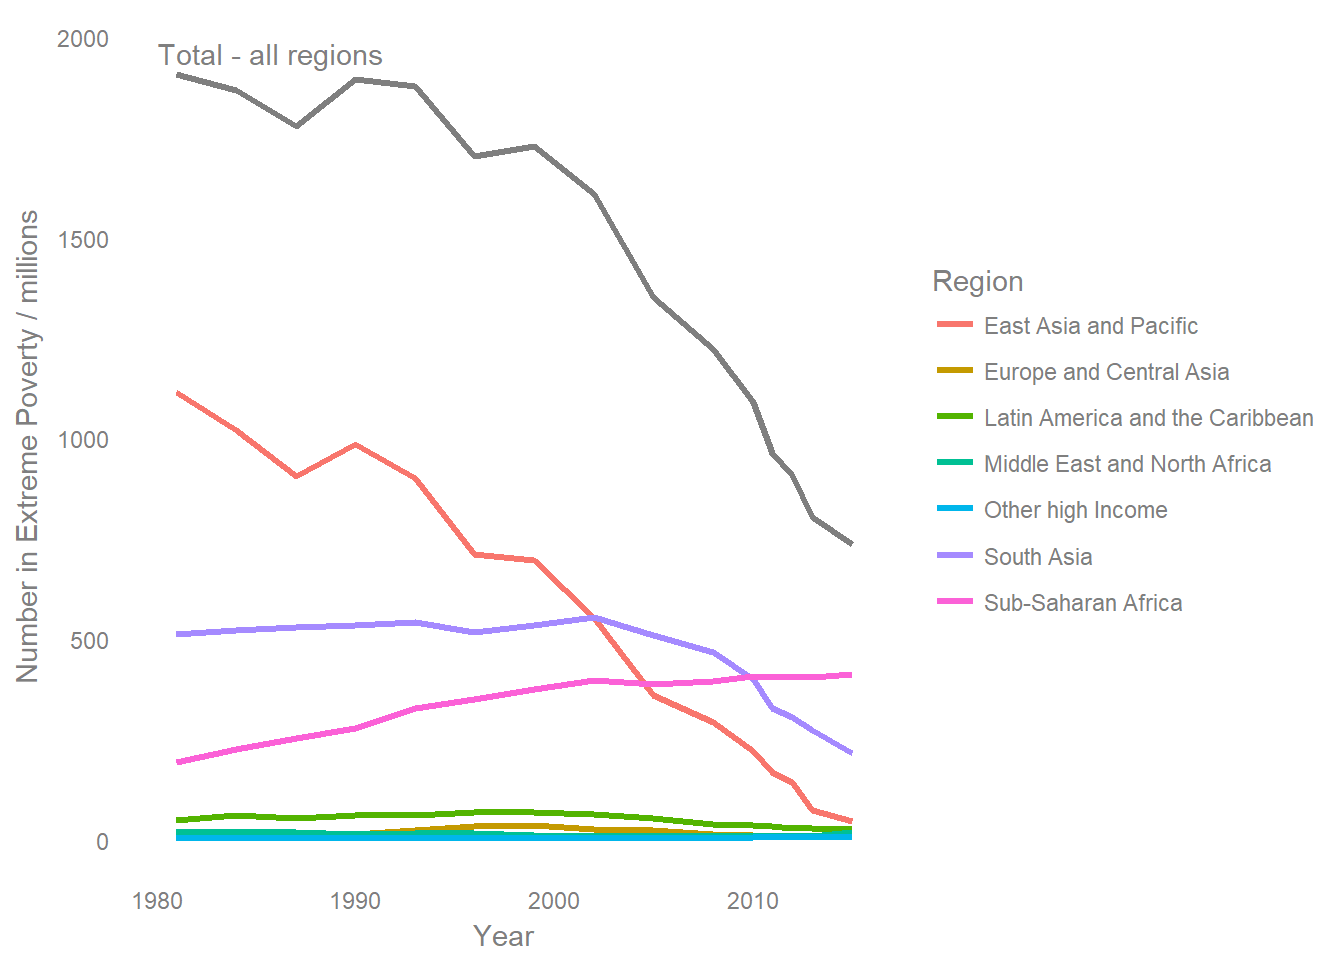
\includegraphics{2018-10-25-replicating-flowingdata-population-charts-in-r_files/figure-latex/unnamed-chunk-5-1.png}

This gives us the right shape, but there looks to be something odd going
on with the jumps. This is due to the variable ``Age Code'' being a
character variable which is turned into a factor by ggplot2 when used as
an x-axis value.

Because factors are being sorted alphabetically you end up with the
projection for 100 near the start, which causes the first spike. We can
confirm this:

\begin{Shaded}
\begin{Highlighting}[]
\KeywordTok{str}\NormalTok{(}\KeywordTok{as.factor}\NormalTok{(chartData}\OperatorTok{$}\StringTok{`}\DataTypeTok{Age Code}\StringTok{`}\NormalTok{))}
\end{Highlighting}
\end{Shaded}

\begin{verbatim}
##  Factor w/ 101 levels "0","1","10","100+",..: 1 1 1 1 1 1 1 1 1 1 ...
\end{verbatim}

As you can see, the third and fourth values of the factor are 10 and
100+ not 2 and 3 as we would want, hence the spikes in the chart.

It's probably easiest to just code this variable as a numeric value, as
text is only needed to signify 100+ which can be dealt with later when
labelling the chart.

\begin{Shaded}
\begin{Highlighting}[]
\NormalTok{chartData }\OperatorTok\StringTok{ }\KeywordTok{ungroup}\NormalTok{() }\OperatorTok\StringTok{ }\KeywordTok{mutate}\NormalTok{(}\StringTok{`}\DataTypeTok{Age Code}\StringTok{`}\NormalTok{=}\KeywordTok{as.numeric}\NormalTok{(}\KeywordTok{str_replace}\NormalTok{(}\StringTok{`}\DataTypeTok{Age Code}\StringTok{`}\NormalTok{,}\StringTok{"}\CharTok{\textbackslash{}\textbackslash{}}\StringTok{+"}\NormalTok{,}\StringTok{""}\NormalTok{))) ->}\StringTok{ }\NormalTok{chartData}
\end{Highlighting}
\end{Shaded}

With those changes made, we can now revist the chart:

\begin{Shaded}
\begin{Highlighting}[]
\NormalTok{chartData }\OperatorTok\StringTok{ }\KeywordTok{filter}\NormalTok{(Year}\OperatorTok{==}\DecValTok{2014}\NormalTok{) }\OperatorTok
\StringTok{  }\KeywordTok{ggplot}\NormalTok{() }\OperatorTok{+}
\StringTok{  }\KeywordTok{geom_ribbon}\NormalTok{(}\KeywordTok{aes}\NormalTok{(}\DataTypeTok{x=}\StringTok{`}\DataTypeTok{Age Code}\StringTok{`}\NormalTok{,}\DataTypeTok{ymin=}\NormalTok{Lower,}\DataTypeTok{ymax=}\NormalTok{Upper)) }
\end{Highlighting}
\end{Shaded}

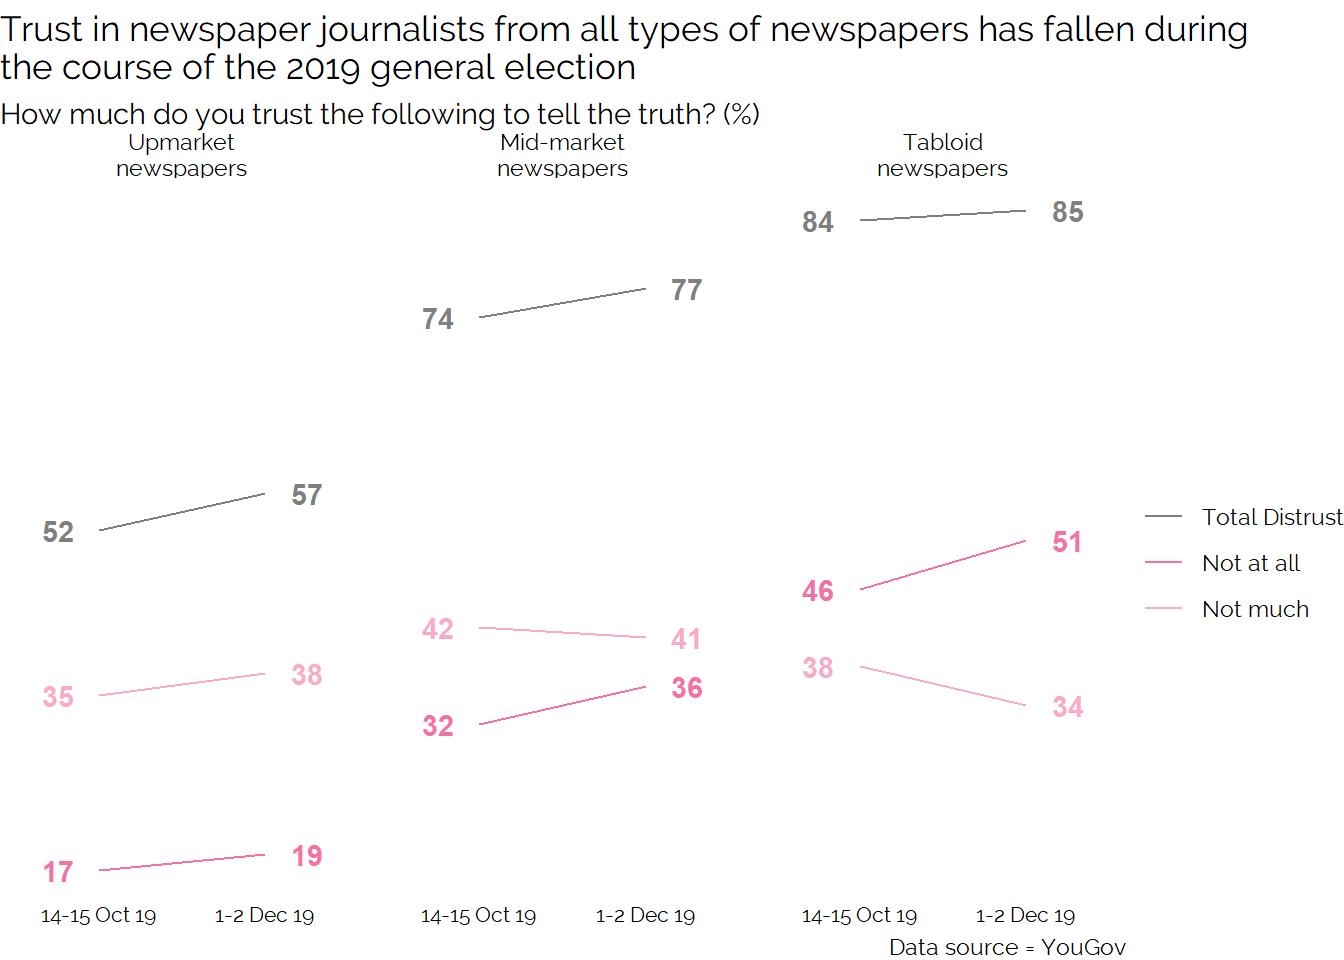
\includegraphics{2018-10-25-replicating-flowingdata-population-charts-in-r_files/figure-latex/unnamed-chunk-8-1.png}

This is now starting to look a bit more promising, we have the right
shape for the graph. Because \texttt{Age\ Code} is now numeric, ggplot2
is also automatically doing some a bit nice looking with the axis
labelling.

Now, let's try to colour the ribbon based on the highest value:

\begin{Shaded}
\begin{Highlighting}[]
\NormalTok{chartData }\OperatorTok\StringTok{ }\KeywordTok{filter}\NormalTok{(Year}\OperatorTok{==}\DecValTok{2014}\NormalTok{) }\OperatorTok
\StringTok{  }\KeywordTok{ggplot}\NormalTok{() }\OperatorTok{+}
\StringTok{  }\KeywordTok{geom_ribbon}\NormalTok{(}\KeywordTok{aes}\NormalTok{(}\DataTypeTok{x=}\StringTok{`}\DataTypeTok{Age Code}\StringTok{`}\NormalTok{,}\DataTypeTok{ymin=}\NormalTok{Lower,}\DataTypeTok{ymax=}\NormalTok{Upper,}\DataTypeTok{fill=}\NormalTok{UpperGender))}
\end{Highlighting}
\end{Shaded}

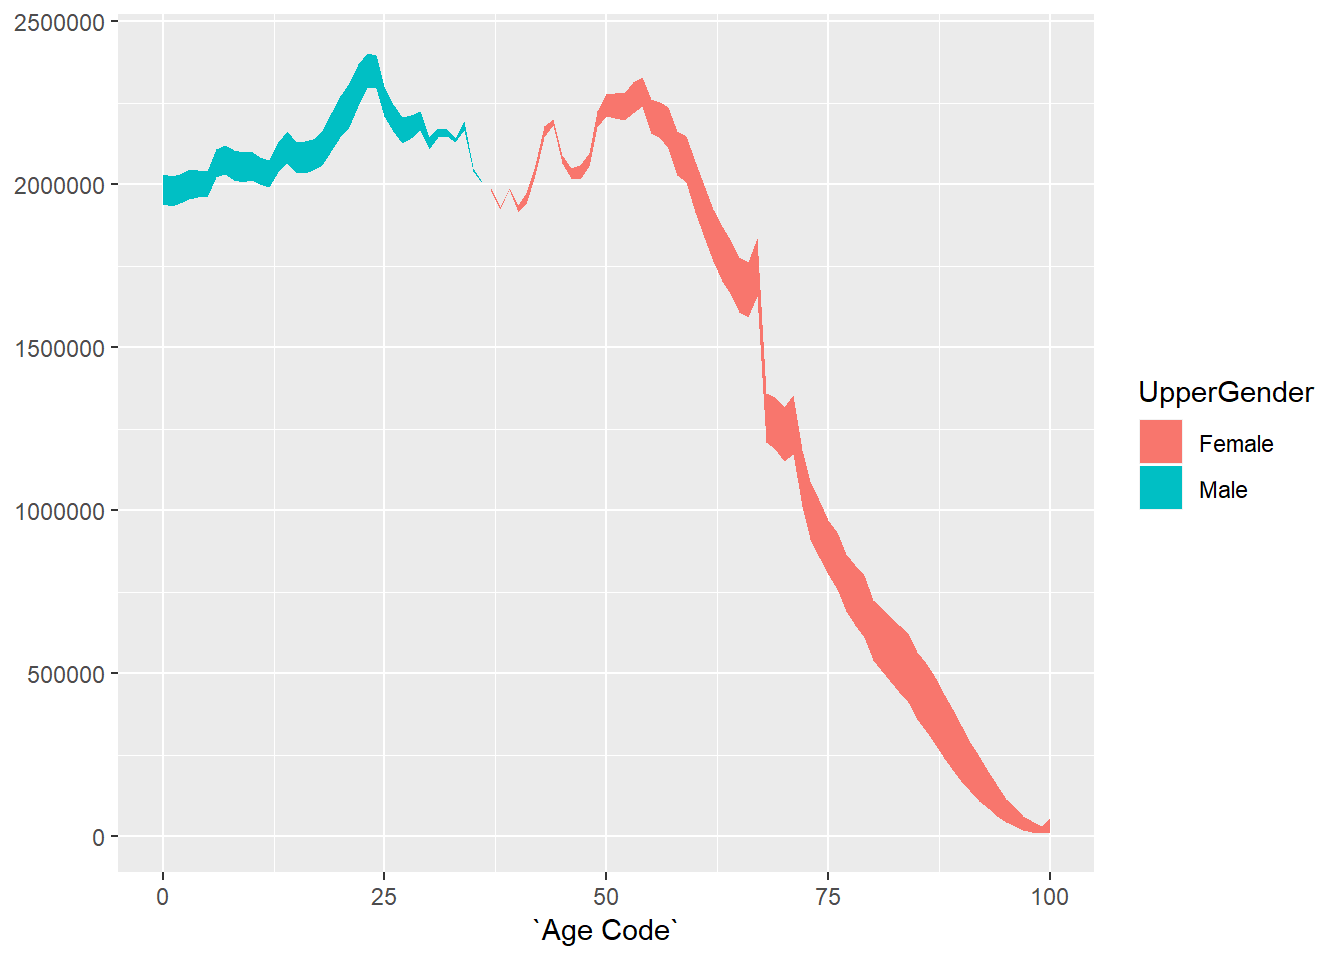
\includegraphics{2018-10-25-replicating-flowingdata-population-charts-in-r_files/figure-latex/unnamed-chunk-9-1.png}

The original plot also has lines bordering the shaded region, so let's
add those using geom\_line:

\begin{Shaded}
\begin{Highlighting}[]
\NormalTok{chartData }\OperatorTok\StringTok{ }\KeywordTok{filter}\NormalTok{(Year}\OperatorTok{==}\DecValTok{2014}\NormalTok{) }\OperatorTok
\StringTok{  }\KeywordTok{ggplot}\NormalTok{() }\OperatorTok{+}
\StringTok{  }\KeywordTok{geom_ribbon}\NormalTok{(}\KeywordTok{aes}\NormalTok{(}\DataTypeTok{x=}\StringTok{`}\DataTypeTok{Age Code}\StringTok{`}\NormalTok{,}\DataTypeTok{ymin=}\NormalTok{Lower,}\DataTypeTok{ymax=}\NormalTok{Upper,}\DataTypeTok{fill=}\NormalTok{UpperGender)) }\OperatorTok{+}
\StringTok{  }\KeywordTok{geom_line}\NormalTok{(}\KeywordTok{aes}\NormalTok{(}\DataTypeTok{x=}\StringTok{`}\DataTypeTok{Age Code}\StringTok{`}\NormalTok{,}\DataTypeTok{y=}\NormalTok{Lower,}\DataTypeTok{colour=}\NormalTok{LowerGender)) }\OperatorTok{+}
\StringTok{  }\KeywordTok{geom_line}\NormalTok{(}\KeywordTok{aes}\NormalTok{(}\DataTypeTok{x=}\StringTok{`}\DataTypeTok{Age Code}\StringTok{`}\NormalTok{,}\DataTypeTok{y=}\NormalTok{Upper,}\DataTypeTok{colour=}\NormalTok{UpperGender))}
\end{Highlighting}
\end{Shaded}

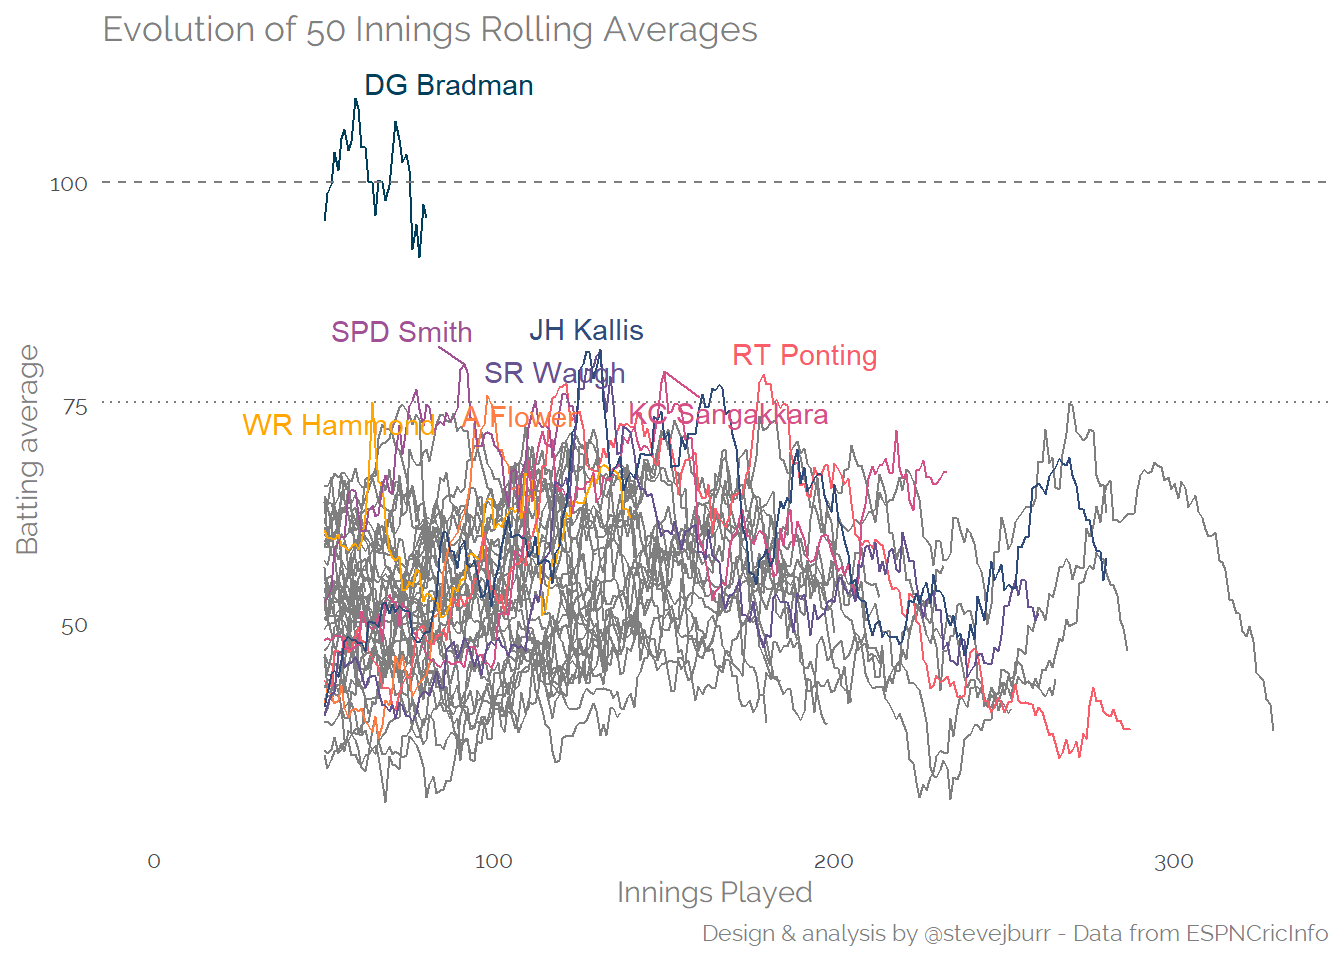
\includegraphics{2018-10-25-replicating-flowingdata-population-charts-in-r_files/figure-latex/unnamed-chunk-10-1.png}

We now have the basic chart that we need, but it doesn't look very
visually appealling, the next step is to do some formatting to get
closer to the original.

\paragraph{Step 3 - Formatting the single year
plot}\label{step-3---formatting-the-single-year-plot}

First let's adjust the axis labelling to match the original:

\begin{Shaded}
\begin{Highlighting}[]
\NormalTok{chartData }\OperatorTok\StringTok{ }\KeywordTok{filter}\NormalTok{(Year}\OperatorTok{==}\DecValTok{2014}\NormalTok{) }\OperatorTok
\StringTok{  }\KeywordTok{ggplot}\NormalTok{() }\OperatorTok{+}
\StringTok{  }\KeywordTok{geom_ribbon}\NormalTok{(}\KeywordTok{aes}\NormalTok{(}\DataTypeTok{x=}\StringTok{`}\DataTypeTok{Age Code}\StringTok{`}\NormalTok{,}\DataTypeTok{ymin=}\NormalTok{Lower,}\DataTypeTok{ymax=}\NormalTok{Upper,}\DataTypeTok{fill=}\NormalTok{UpperGender)) }\OperatorTok{+}
\StringTok{  }\KeywordTok{geom_line}\NormalTok{(}\KeywordTok{aes}\NormalTok{(}\DataTypeTok{x=}\StringTok{`}\DataTypeTok{Age Code}\StringTok{`}\NormalTok{,}\DataTypeTok{y=}\NormalTok{Lower,}\DataTypeTok{colour=}\NormalTok{LowerGender)) }\OperatorTok{+}
\StringTok{  }\KeywordTok{geom_line}\NormalTok{(}\KeywordTok{aes}\NormalTok{(}\DataTypeTok{x=}\StringTok{`}\DataTypeTok{Age Code}\StringTok{`}\NormalTok{,}\DataTypeTok{y=}\NormalTok{Upper,}\DataTypeTok{colour=}\NormalTok{UpperGender)) }\OperatorTok{+}
\StringTok{  }\KeywordTok{scale_y_continuous}\NormalTok{(}\StringTok{"POPULATION"}\NormalTok{, }\CommentTok{#the title for the axis}
                     \DataTypeTok{limits=}\KeywordTok{c}\NormalTok{(}\DecValTok{0}\NormalTok{,}\DecValTok{3000000}\NormalTok{), }\CommentTok{#set the top and bottom value}
                     \DataTypeTok{expand=}\KeywordTok{c}\NormalTok{(}\DecValTok{0}\NormalTok{,}\DecValTok{0}\NormalTok{), }\CommentTok{#don't expand beyond the specified limits}
                     \DataTypeTok{breaks=}\KeywordTok{c}\NormalTok{(}\DecValTok{0}\NormalTok{,}\DecValTok{500000}\NormalTok{,}\DecValTok{1000000}\NormalTok{,}\DecValTok{1500000}\NormalTok{,}\DecValTok{2000000}\NormalTok{,}\DecValTok{2500000}\NormalTok{,}\DecValTok{3000000}\NormalTok{), }\CommentTok{#specify what to put on the axis}
                     \DataTypeTok{labels=}\NormalTok{scales}\OperatorTok{::}\KeywordTok{comma_format}\NormalTok{(}\DataTypeTok{scale=}\FloatTok{0.001}\NormalTok{,}\DataTypeTok{suffix=}\StringTok{"k"}\NormalTok{)) }\OperatorTok{+}\StringTok{ }\CommentTok{# format the displayed numbers using the scales package}
\StringTok{  }\KeywordTok{scale_x_continuous}\NormalTok{(}\StringTok{"AGE"}\NormalTok{, }\CommentTok{#axis title}
                     \DataTypeTok{breaks=} \KeywordTok{c}\NormalTok{(}\DecValTok{0}\NormalTok{,}\DecValTok{10}\NormalTok{,}\DecValTok{20}\NormalTok{,}\DecValTok{30}\NormalTok{,}\DecValTok{40}\NormalTok{,}\DecValTok{50}\NormalTok{,}\DecValTok{60}\NormalTok{,}\DecValTok{70}\NormalTok{,}\DecValTok{80}\NormalTok{,}\DecValTok{90}\NormalTok{,}\DecValTok{100}\NormalTok{),}
                     \DataTypeTok{labels=}\KeywordTok{c}\NormalTok{(}\StringTok{"0"}\NormalTok{,}\StringTok{"10"}\NormalTok{,}\StringTok{"20"}\NormalTok{,}\StringTok{"30"}\NormalTok{,}\StringTok{"40"}\NormalTok{,}\StringTok{"50"}\NormalTok{,}\StringTok{"60"}\NormalTok{,}\StringTok{"70"}\NormalTok{,}\StringTok{"80"}\NormalTok{,}\StringTok{"90"}\NormalTok{,}\StringTok{"100+"}\NormalTok{)) }\OperatorTok{+}
\StringTok{  }\KeywordTok{theme}\NormalTok{(}\DataTypeTok{text=}\KeywordTok{element_text}\NormalTok{(}\DataTypeTok{colour=}\StringTok{"black"}\NormalTok{), }\CommentTok{#all text is black}
        \DataTypeTok{axis.text =} \KeywordTok{element_text}\NormalTok{(}\DataTypeTok{colour=}\StringTok{"black"}\NormalTok{), }\CommentTok{#make sure labels are black also}
        \DataTypeTok{axis.title.y=}\KeywordTok{element_text}\NormalTok{(}\DataTypeTok{vjust=}\DecValTok{1}\NormalTok{,}\DataTypeTok{angle=}\DecValTok{0}\NormalTok{), }\CommentTok{#move the label of the y to the top and don't rotate it}
        \DataTypeTok{axis.title.x=}\KeywordTok{element_text}\NormalTok{(}\DataTypeTok{hjust=}\DecValTok{0}\NormalTok{,}\DataTypeTok{angle=}\DecValTok{0}\NormalTok{)) }\CommentTok{#move the label of the x axis to the left and don't rotate it}
\end{Highlighting}
\end{Shaded}

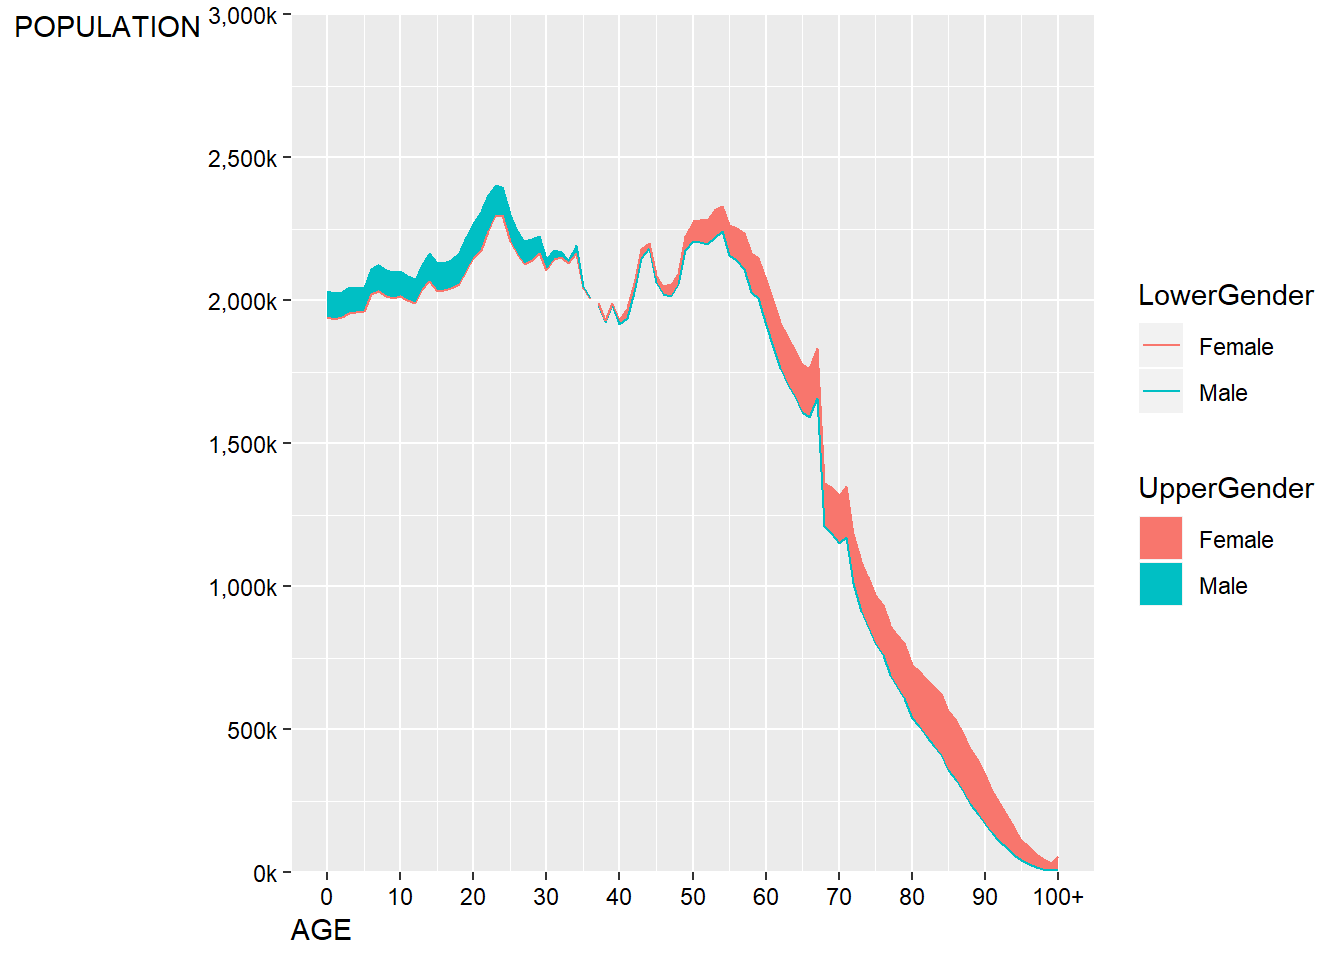
\includegraphics{2018-10-25-replicating-flowingdata-population-charts-in-r_files/figure-latex/unnamed-chunk-11-1.png}

This is fairly close, but it doesn't quite get the y-axis label in the
right place. As there's no title on this plot, we can cheat slightly and
just use a left aligned subtitle to the plot to play the role of a
y-axis label.

\begin{Shaded}
\begin{Highlighting}[]
\NormalTok{chartData }\OperatorTok\StringTok{ }\KeywordTok{filter}\NormalTok{(Year}\OperatorTok{==}\DecValTok{2014}\NormalTok{) }\OperatorTok
\StringTok{  }\KeywordTok{ggplot}\NormalTok{() }\OperatorTok{+}
\StringTok{  }\KeywordTok{geom_ribbon}\NormalTok{(}\KeywordTok{aes}\NormalTok{(}\DataTypeTok{x=}\StringTok{`}\DataTypeTok{Age Code}\StringTok{`}\NormalTok{,}\DataTypeTok{ymin=}\NormalTok{Lower,}\DataTypeTok{ymax=}\NormalTok{Upper,}\DataTypeTok{fill=}\NormalTok{UpperGender)) }\OperatorTok{+}
\StringTok{  }\KeywordTok{geom_line}\NormalTok{(}\KeywordTok{aes}\NormalTok{(}\DataTypeTok{x=}\StringTok{`}\DataTypeTok{Age Code}\StringTok{`}\NormalTok{,}\DataTypeTok{y=}\NormalTok{Lower,}\DataTypeTok{colour=}\NormalTok{LowerGender)) }\OperatorTok{+}
\StringTok{  }\KeywordTok{geom_line}\NormalTok{(}\KeywordTok{aes}\NormalTok{(}\DataTypeTok{x=}\StringTok{`}\DataTypeTok{Age Code}\StringTok{`}\NormalTok{,}\DataTypeTok{y=}\NormalTok{Upper,}\DataTypeTok{colour=}\NormalTok{UpperGender)) }\OperatorTok{+}
\StringTok{  }\KeywordTok{scale_y_continuous}\NormalTok{(}\StringTok{""}\NormalTok{, }\CommentTok{#the title for the axis}
                     \DataTypeTok{limits=}\KeywordTok{c}\NormalTok{(}\DecValTok{0}\NormalTok{,}\DecValTok{3000000}\NormalTok{), }\CommentTok{#set the top and bottom value}
                     \DataTypeTok{expand=}\KeywordTok{c}\NormalTok{(}\DecValTok{0}\NormalTok{,}\DecValTok{0}\NormalTok{), }\CommentTok{#don't expand beyond the specified limits}
                     \DataTypeTok{breaks=}\KeywordTok{c}\NormalTok{(}\DecValTok{0}\NormalTok{,}\DecValTok{500000}\NormalTok{,}\DecValTok{1000000}\NormalTok{,}\DecValTok{1500000}\NormalTok{,}\DecValTok{2000000}\NormalTok{,}\DecValTok{2500000}\NormalTok{,}\DecValTok{3000000}\NormalTok{), }\CommentTok{#specify what to put on the axis}
                     \DataTypeTok{labels=}\NormalTok{scales}\OperatorTok{::}\KeywordTok{comma_format}\NormalTok{(}\DataTypeTok{scale=}\FloatTok{0.001}\NormalTok{,}\DataTypeTok{suffix=}\StringTok{"k"}\NormalTok{)) }\OperatorTok{+}\StringTok{ }\CommentTok{# format the displayed numbers using the scales package}
\StringTok{  }\KeywordTok{scale_x_continuous}\NormalTok{(}\StringTok{"AGE"}\NormalTok{, }\CommentTok{#axis title}
                     \DataTypeTok{breaks=} \KeywordTok{c}\NormalTok{(}\DecValTok{0}\NormalTok{,}\DecValTok{10}\NormalTok{,}\DecValTok{20}\NormalTok{,}\DecValTok{30}\NormalTok{,}\DecValTok{40}\NormalTok{,}\DecValTok{50}\NormalTok{,}\DecValTok{60}\NormalTok{,}\DecValTok{70}\NormalTok{,}\DecValTok{80}\NormalTok{,}\DecValTok{90}\NormalTok{,}\DecValTok{100}\NormalTok{),}
                     \DataTypeTok{labels=}\KeywordTok{c}\NormalTok{(}\StringTok{"0"}\NormalTok{,}\StringTok{"10"}\NormalTok{,}\StringTok{"20"}\NormalTok{,}\StringTok{"30"}\NormalTok{,}\StringTok{"40"}\NormalTok{,}\StringTok{"50"}\NormalTok{,}\StringTok{"60"}\NormalTok{,}\StringTok{"70"}\NormalTok{,}\StringTok{"80"}\NormalTok{,}\StringTok{"90"}\NormalTok{,}\StringTok{"100+"}\NormalTok{)) }\OperatorTok{+}
\StringTok{  }\KeywordTok{labs}\NormalTok{(}\DataTypeTok{subtitle=}\StringTok{"POPULATION"}\NormalTok{)}\OperatorTok{+}
\StringTok{  }\KeywordTok{theme}\NormalTok{(}\DataTypeTok{text=}\KeywordTok{element_text}\NormalTok{(}\DataTypeTok{colour=}\StringTok{"black"}\NormalTok{), }\CommentTok{#all text is black}
        \DataTypeTok{plot.subtitle=}\KeywordTok{element_text}\NormalTok{(}\DataTypeTok{size=}\DecValTok{9}\NormalTok{),}
        \DataTypeTok{axis.text =} \KeywordTok{element_text}\NormalTok{(}\DataTypeTok{colour=}\StringTok{"black"}\NormalTok{), }\CommentTok{#make sure labels are black also}
        \DataTypeTok{axis.title.x=}\KeywordTok{element_text}\NormalTok{(}\DataTypeTok{hjust=}\DecValTok{0}\NormalTok{,}\DataTypeTok{angle=}\DecValTok{0}\NormalTok{)) }\CommentTok{#move the label of the x axis to the left and don't rotate it}
\end{Highlighting}
\end{Shaded}

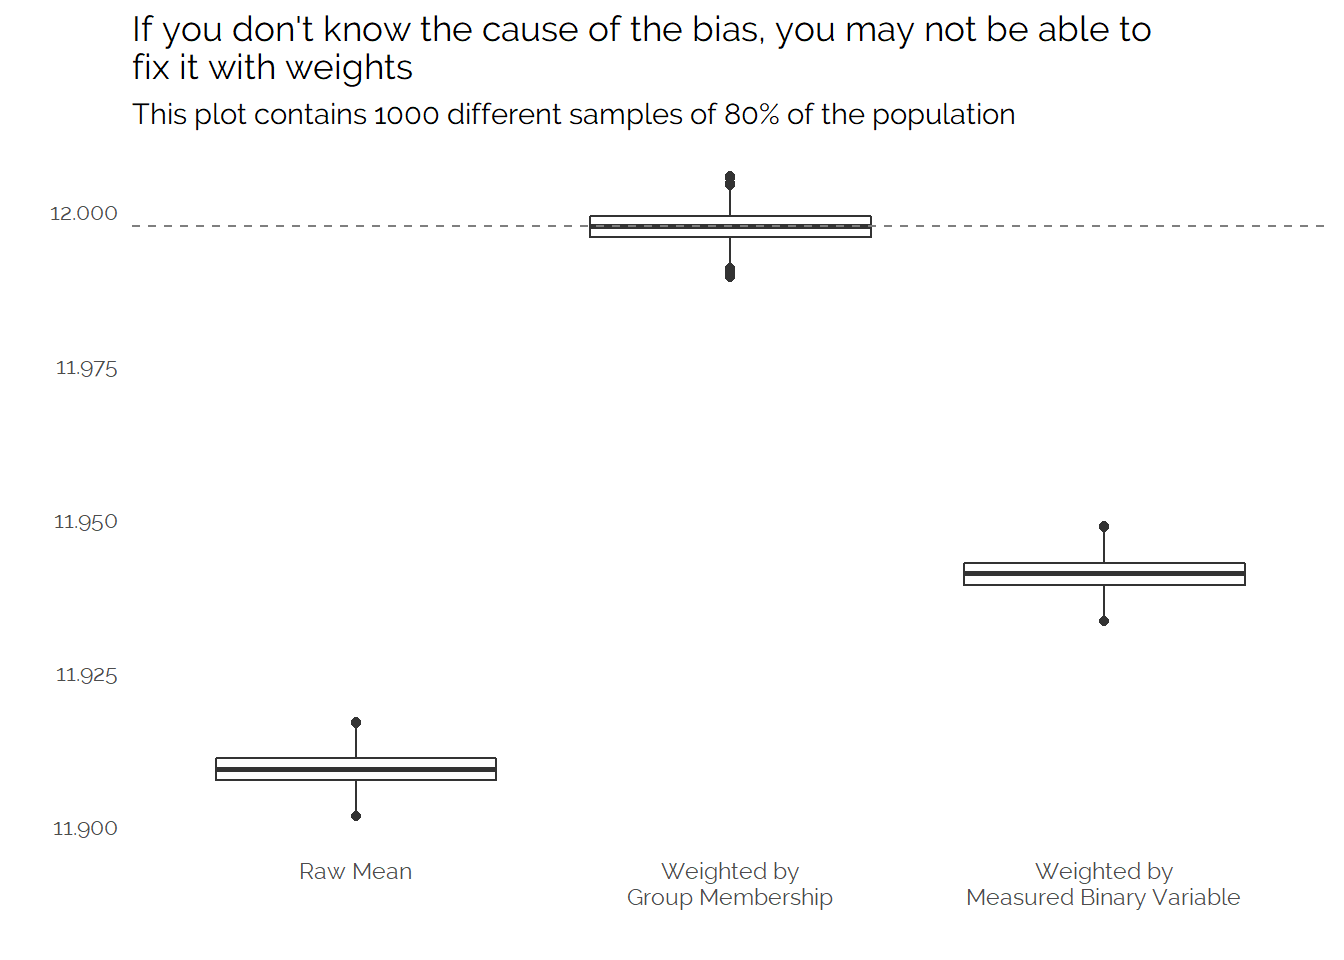
\includegraphics{2018-10-25-replicating-flowingdata-population-charts-in-r_files/figure-latex/unnamed-chunk-12-1.png}

This still isn't quite what we want - it's currently left algined to the
axis not the plot edge, this can be manually adjusted:

\begin{Shaded}
\begin{Highlighting}[]
\NormalTok{chartData }\OperatorTok\StringTok{ }\KeywordTok{filter}\NormalTok{(Year}\OperatorTok{==}\DecValTok{2014}\NormalTok{) }\OperatorTok
\StringTok{  }\KeywordTok{ggplot}\NormalTok{() }\OperatorTok{+}
\StringTok{  }\KeywordTok{geom_ribbon}\NormalTok{(}\KeywordTok{aes}\NormalTok{(}\DataTypeTok{x=}\StringTok{`}\DataTypeTok{Age Code}\StringTok{`}\NormalTok{,}\DataTypeTok{ymin=}\NormalTok{Lower,}\DataTypeTok{ymax=}\NormalTok{Upper,}\DataTypeTok{fill=}\NormalTok{UpperGender)) }\OperatorTok{+}
\StringTok{  }\KeywordTok{geom_line}\NormalTok{(}\KeywordTok{aes}\NormalTok{(}\DataTypeTok{x=}\StringTok{`}\DataTypeTok{Age Code}\StringTok{`}\NormalTok{,}\DataTypeTok{y=}\NormalTok{Lower,}\DataTypeTok{colour=}\NormalTok{LowerGender)) }\OperatorTok{+}
\StringTok{  }\KeywordTok{geom_line}\NormalTok{(}\KeywordTok{aes}\NormalTok{(}\DataTypeTok{x=}\StringTok{`}\DataTypeTok{Age Code}\StringTok{`}\NormalTok{,}\DataTypeTok{y=}\NormalTok{Upper,}\DataTypeTok{colour=}\NormalTok{UpperGender)) }\OperatorTok{+}
\StringTok{  }\KeywordTok{scale_y_continuous}\NormalTok{(}\StringTok{""}\NormalTok{, }\CommentTok{#the title for the axis}
                     \DataTypeTok{limits=}\KeywordTok{c}\NormalTok{(}\DecValTok{0}\NormalTok{,}\DecValTok{3000000}\NormalTok{), }\CommentTok{#set the top and bottom value}
                     \DataTypeTok{expand=}\KeywordTok{c}\NormalTok{(}\DecValTok{0}\NormalTok{,}\DecValTok{0}\NormalTok{), }\CommentTok{#don't expand beyond the specified limits}
                     \DataTypeTok{breaks=}\KeywordTok{c}\NormalTok{(}\DecValTok{0}\NormalTok{,}\DecValTok{500000}\NormalTok{,}\DecValTok{1000000}\NormalTok{,}\DecValTok{1500000}\NormalTok{,}\DecValTok{2000000}\NormalTok{,}\DecValTok{2500000}\NormalTok{,}\DecValTok{3000000}\NormalTok{), }\CommentTok{#specify what to put on the axis}
                     \DataTypeTok{labels=}\NormalTok{scales}\OperatorTok{::}\KeywordTok{comma_format}\NormalTok{(}\DataTypeTok{scale=}\FloatTok{0.001}\NormalTok{,}\DataTypeTok{suffix=}\StringTok{"k"}\NormalTok{)) }\OperatorTok{+}\StringTok{ }\CommentTok{# format the displayed numbers using the scales package}
\StringTok{  }\KeywordTok{scale_x_continuous}\NormalTok{(}\StringTok{"AGE"}\NormalTok{, }\CommentTok{#axis title}
                     \DataTypeTok{breaks=} \KeywordTok{c}\NormalTok{(}\DecValTok{0}\NormalTok{,}\DecValTok{10}\NormalTok{,}\DecValTok{20}\NormalTok{,}\DecValTok{30}\NormalTok{,}\DecValTok{40}\NormalTok{,}\DecValTok{50}\NormalTok{,}\DecValTok{60}\NormalTok{,}\DecValTok{70}\NormalTok{,}\DecValTok{80}\NormalTok{,}\DecValTok{90}\NormalTok{,}\DecValTok{100}\NormalTok{),}
                     \DataTypeTok{labels=}\KeywordTok{c}\NormalTok{(}\StringTok{"0"}\NormalTok{,}\StringTok{"10"}\NormalTok{,}\StringTok{"20"}\NormalTok{,}\StringTok{"30"}\NormalTok{,}\StringTok{"40"}\NormalTok{,}\StringTok{"50"}\NormalTok{,}\StringTok{"60"}\NormalTok{,}\StringTok{"70"}\NormalTok{,}\StringTok{"80"}\NormalTok{,}\StringTok{"90"}\NormalTok{,}\StringTok{"100+"}\NormalTok{)) }\OperatorTok{+}
\StringTok{  }\KeywordTok{labs}\NormalTok{(}\DataTypeTok{subtitle=}\StringTok{"POPULATION"}\NormalTok{)}\OperatorTok{+}
\StringTok{  }\KeywordTok{theme}\NormalTok{(}\DataTypeTok{text=}\KeywordTok{element_text}\NormalTok{(}\DataTypeTok{colour=}\StringTok{"black"}\NormalTok{), }\CommentTok{#all text is black}
        \DataTypeTok{plot.subtitle=}\KeywordTok{element_text}\NormalTok{(}\DataTypeTok{size=}\DecValTok{9}\NormalTok{),}
        \DataTypeTok{axis.text =} \KeywordTok{element_text}\NormalTok{(}\DataTypeTok{colour=}\StringTok{"black"}\NormalTok{), }\CommentTok{#make sure labels are black also}
        \DataTypeTok{axis.title.x=}\KeywordTok{element_text}\NormalTok{(}\DataTypeTok{hjust=}\DecValTok{0}\NormalTok{,}\DataTypeTok{angle=}\DecValTok{0}\NormalTok{,}\DataTypeTok{size=}\DecValTok{9}\NormalTok{)) ->}\StringTok{ }\NormalTok{p }\CommentTok{#move the label of the x axis to the left and don't rotate it }

\CommentTok{#turn the plot into a gtable object}
\NormalTok{g <-}\StringTok{ }\KeywordTok{ggplotGrob}\NormalTok{(p)}
\CommentTok{#adjust the position of the subtitle}
\NormalTok{g}\OperatorTok{$}\NormalTok{layout}\OperatorTok{$}\NormalTok{l[g}\OperatorTok{$}\NormalTok{layout}\OperatorTok{$}\NormalTok{name }\OperatorTok{==}\StringTok{ "subtitle"}\NormalTok{] <-}\StringTok{ }\DecValTok{1}
\CommentTok{#draw the new plot}
\NormalTok{grid}\OperatorTok{::}\KeywordTok{grid.draw}\NormalTok{(g)}
\end{Highlighting}
\end{Shaded}

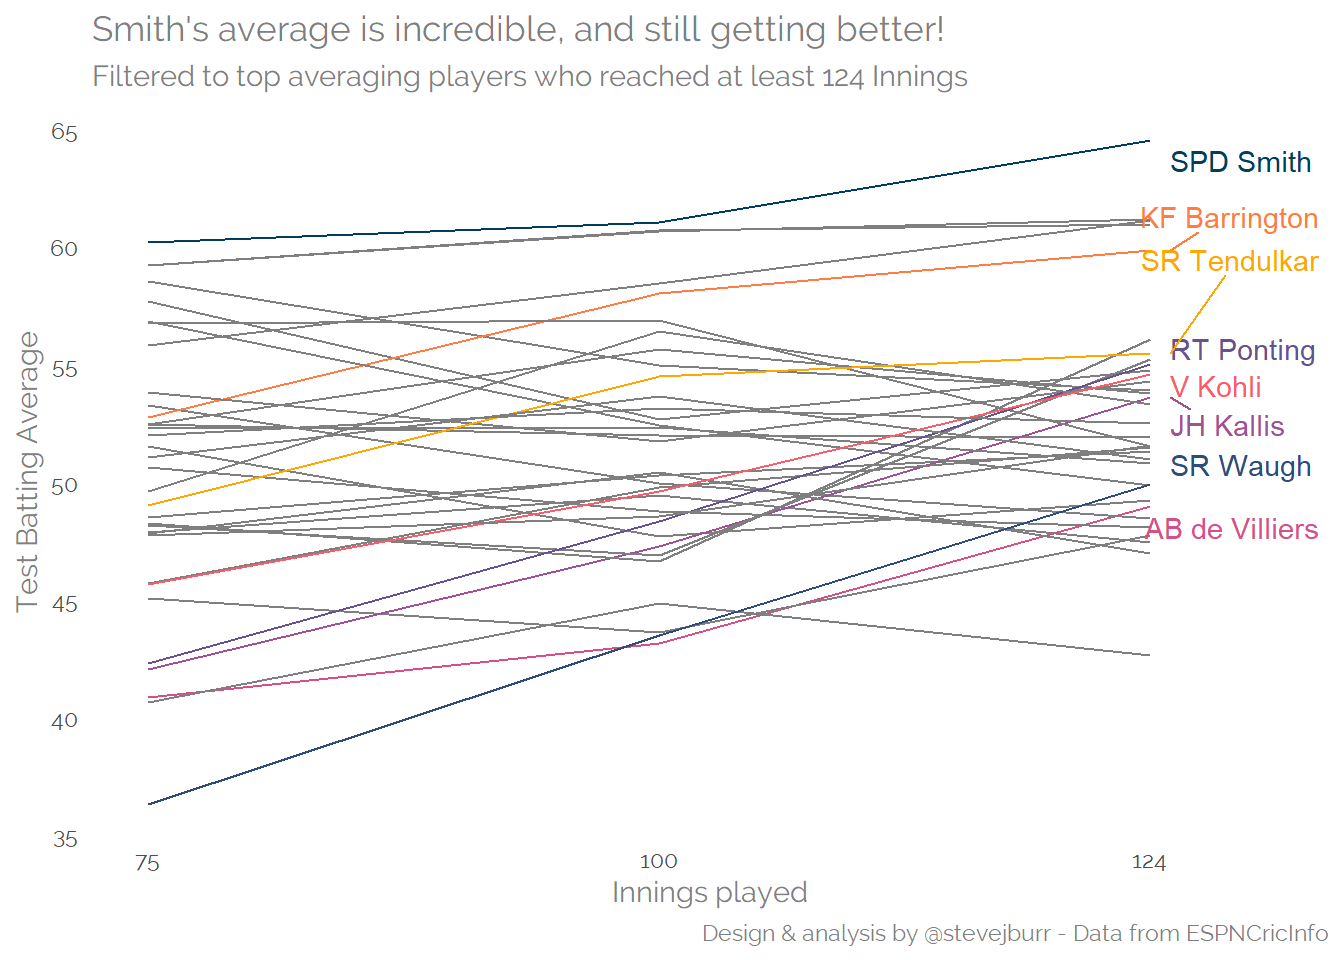
\includegraphics{2018-10-25-replicating-flowingdata-population-charts-in-r_files/figure-latex/unnamed-chunk-13-1.png}

This is close enough for now, precise positioning and alignments of
objects within ggplot2 can often be quite time consuming which is why a
lot of people choose to incorporate Adobe Illustrator into their
workflows in order to add the finishing touches.

Next I'll adjust the general style of the plot so that it is a bit
clearer:

\begin{Shaded}
\begin{Highlighting}[]
\NormalTok{chartData }\OperatorTok\StringTok{ }\KeywordTok{filter}\NormalTok{(Year}\OperatorTok{==}\DecValTok{2014}\NormalTok{) }\OperatorTok
\StringTok{  }\KeywordTok{ggplot}\NormalTok{() }\OperatorTok{+}
\StringTok{  }\KeywordTok{geom_ribbon}\NormalTok{(}\KeywordTok{aes}\NormalTok{(}\DataTypeTok{x=}\StringTok{`}\DataTypeTok{Age Code}\StringTok{`}\NormalTok{,}\DataTypeTok{ymin=}\NormalTok{Lower,}\DataTypeTok{ymax=}\NormalTok{Upper,}\DataTypeTok{fill=}\NormalTok{UpperGender)) }\OperatorTok{+}
\StringTok{  }\KeywordTok{geom_line}\NormalTok{(}\KeywordTok{aes}\NormalTok{(}\DataTypeTok{x=}\StringTok{`}\DataTypeTok{Age Code}\StringTok{`}\NormalTok{,}\DataTypeTok{y=}\NormalTok{Lower,}\DataTypeTok{colour=}\NormalTok{LowerGender)) }\OperatorTok{+}
\StringTok{  }\KeywordTok{geom_line}\NormalTok{(}\KeywordTok{aes}\NormalTok{(}\DataTypeTok{x=}\StringTok{`}\DataTypeTok{Age Code}\StringTok{`}\NormalTok{,}\DataTypeTok{y=}\NormalTok{Upper,}\DataTypeTok{colour=}\NormalTok{UpperGender)) }\OperatorTok{+}
\StringTok{  }\KeywordTok{scale_y_continuous}\NormalTok{(}\StringTok{""}\NormalTok{, }\CommentTok{#the title for the axis}
                     \DataTypeTok{limits=}\KeywordTok{c}\NormalTok{(}\DecValTok{0}\NormalTok{,}\DecValTok{3000000}\NormalTok{), }\CommentTok{#set the top and bottom value}
                     \DataTypeTok{expand=}\KeywordTok{c}\NormalTok{(}\DecValTok{0}\NormalTok{,}\DecValTok{0}\NormalTok{), }\CommentTok{#don't expand beyond the specified limits}
                     \DataTypeTok{breaks=}\KeywordTok{c}\NormalTok{(}\DecValTok{0}\NormalTok{,}\DecValTok{500000}\NormalTok{,}\DecValTok{1000000}\NormalTok{,}\DecValTok{1500000}\NormalTok{,}\DecValTok{2000000}\NormalTok{,}\DecValTok{2500000}\NormalTok{,}\DecValTok{3000000}\NormalTok{), }\CommentTok{#specify what to put on the axis}
                     \DataTypeTok{labels=}\NormalTok{scales}\OperatorTok{::}\KeywordTok{comma_format}\NormalTok{(}\DataTypeTok{scale=}\FloatTok{0.001}\NormalTok{,}\DataTypeTok{suffix=}\StringTok{"k"}\NormalTok{)) }\OperatorTok{+}\StringTok{ }\CommentTok{# format the displayed numbers using the scales package}
\StringTok{  }\KeywordTok{scale_x_continuous}\NormalTok{(}\StringTok{"AGE"}\NormalTok{, }\CommentTok{#axis title}
                     \DataTypeTok{breaks=} \KeywordTok{c}\NormalTok{(}\DecValTok{0}\NormalTok{,}\DecValTok{10}\NormalTok{,}\DecValTok{20}\NormalTok{,}\DecValTok{30}\NormalTok{,}\DecValTok{40}\NormalTok{,}\DecValTok{50}\NormalTok{,}\DecValTok{60}\NormalTok{,}\DecValTok{70}\NormalTok{,}\DecValTok{80}\NormalTok{,}\DecValTok{90}\NormalTok{,}\DecValTok{100}\NormalTok{),}
                     \DataTypeTok{labels=}\KeywordTok{c}\NormalTok{(}\StringTok{"0"}\NormalTok{,}\StringTok{"10"}\NormalTok{,}\StringTok{"20"}\NormalTok{,}\StringTok{"30"}\NormalTok{,}\StringTok{"40"}\NormalTok{,}\StringTok{"50"}\NormalTok{,}\StringTok{"60"}\NormalTok{,}\StringTok{"70"}\NormalTok{,}\StringTok{"80"}\NormalTok{,}\StringTok{"90"}\NormalTok{,}\StringTok{"100+"}\NormalTok{)) }\OperatorTok{+}
\StringTok{  }\KeywordTok{labs}\NormalTok{(}\DataTypeTok{subtitle=}\StringTok{"POPULATION"}\NormalTok{)}\OperatorTok{+}
\StringTok{  }\KeywordTok{theme_minimal}\NormalTok{() }\OperatorTok{+}\StringTok{ }\CommentTok{#apply my prefered theme which is close to what Nathan used}
\StringTok{  }\KeywordTok{theme}\NormalTok{(}\DataTypeTok{text=}\KeywordTok{element_text}\NormalTok{(}\DataTypeTok{colour=}\StringTok{"black"}\NormalTok{), }\CommentTok{#all text is black}
        \DataTypeTok{plot.subtitle=}\KeywordTok{element_text}\NormalTok{(}\DataTypeTok{size=}\DecValTok{9}\NormalTok{),}
        \DataTypeTok{axis.text =} \KeywordTok{element_text}\NormalTok{(}\DataTypeTok{colour=}\StringTok{"black"}\NormalTok{), }\CommentTok{#make sure labels are black also}
        \DataTypeTok{axis.title.x=}\KeywordTok{element_text}\NormalTok{(}\DataTypeTok{hjust=}\DecValTok{0}\NormalTok{,}\DataTypeTok{angle=}\DecValTok{0}\NormalTok{,}\DataTypeTok{size=}\DecValTok{9}\NormalTok{),}
        \DataTypeTok{panel.grid.minor.x=}\KeywordTok{element_blank}\NormalTok{(), }\CommentTok{#turn off minor gridlines}
        \DataTypeTok{panel.grid.minor.y=}\KeywordTok{element_blank}\NormalTok{(), }\CommentTok{#turn off minor gridlines}
\NormalTok{        ) ->}\StringTok{ }\NormalTok{p}

\CommentTok{#turn the plot into a gtable object}
\NormalTok{g <-}\StringTok{ }\KeywordTok{ggplotGrob}\NormalTok{(p)}
\CommentTok{#adjust the position of the subtitle}
\NormalTok{g}\OperatorTok{$}\NormalTok{layout}\OperatorTok{$}\NormalTok{l[g}\OperatorTok{$}\NormalTok{layout}\OperatorTok{$}\NormalTok{name }\OperatorTok{==}\StringTok{ "subtitle"}\NormalTok{] <-}\StringTok{ }\DecValTok{1}
\CommentTok{#draw the new plot}
\NormalTok{grid}\OperatorTok{::}\KeywordTok{grid.draw}\NormalTok{(g)}
\end{Highlighting}
\end{Shaded}

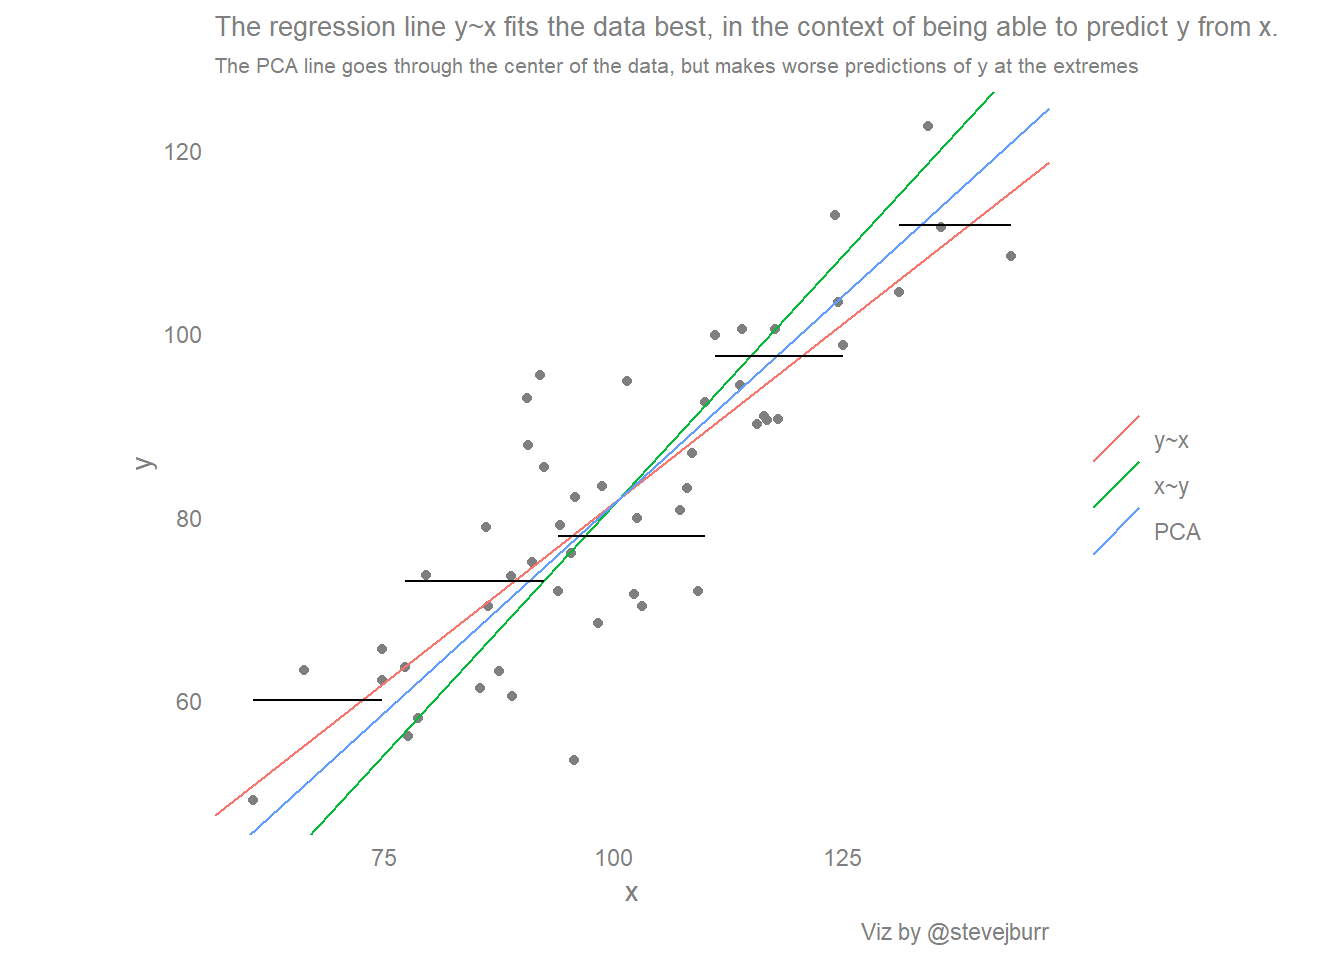
\includegraphics{2018-10-25-replicating-flowingdata-population-charts-in-r_files/figure-latex/unnamed-chunk-14-1.png}

This looks pretty good - the next step is to adjust the colours so they
match the original and sort out the legends.

\begin{Shaded}
\begin{Highlighting}[]
\NormalTok{chartData }\OperatorTok\StringTok{ }\KeywordTok{filter}\NormalTok{(Year}\OperatorTok{==}\DecValTok{2014}\NormalTok{) }\OperatorTok
\StringTok{  }\KeywordTok{ggplot}\NormalTok{() }\OperatorTok{+}
\StringTok{  }\KeywordTok{geom_ribbon}\NormalTok{(}\KeywordTok{aes}\NormalTok{(}\DataTypeTok{x=}\StringTok{`}\DataTypeTok{Age Code}\StringTok{`}\NormalTok{,}\DataTypeTok{ymin=}\NormalTok{Lower,}\DataTypeTok{ymax=}\NormalTok{Upper,}\DataTypeTok{fill=}\NormalTok{UpperGender)) }\OperatorTok{+}
\StringTok{  }\KeywordTok{geom_line}\NormalTok{(}\KeywordTok{aes}\NormalTok{(}\DataTypeTok{x=}\StringTok{`}\DataTypeTok{Age Code}\StringTok{`}\NormalTok{,}\DataTypeTok{y=}\NormalTok{Lower,}\DataTypeTok{colour=}\NormalTok{LowerGender),}\DataTypeTok{show.legend =} \OtherTok{FALSE}\NormalTok{) }\OperatorTok{+}\StringTok{ }
\StringTok{  }\KeywordTok{geom_line}\NormalTok{(}\KeywordTok{aes}\NormalTok{(}\DataTypeTok{x=}\StringTok{`}\DataTypeTok{Age Code}\StringTok{`}\NormalTok{,}\DataTypeTok{y=}\NormalTok{Upper,}\DataTypeTok{colour=}\NormalTok{UpperGender),}\DataTypeTok{show.legend =} \OtherTok{FALSE}\NormalTok{) }\OperatorTok{+}\StringTok{ }\CommentTok{#we don't need the line colours to have a legend}
\StringTok{  }\KeywordTok{scale_fill_manual}\NormalTok{(}\StringTok{""}\NormalTok{,}\CommentTok{#don't label the legend}
                    \DataTypeTok{breaks=}\KeywordTok{c}\NormalTok{(}\StringTok{"Male"}\NormalTok{,}\StringTok{"Female"}\NormalTok{), }\CommentTok{#choose the order to display in }
                    \DataTypeTok{labels=}\KeywordTok{c}\NormalTok{(}\StringTok{"More Men"}\NormalTok{,}\StringTok{"More Women"}\NormalTok{), }\CommentTok{#match the labelling used in the original}
                    \DataTypeTok{values=}\KeywordTok{c}\NormalTok{(women,men), }\CommentTok{#colours to use, in the order of the factor not displayed order}
                    \DataTypeTok{aesthetics =} \KeywordTok{c}\NormalTok{(}\StringTok{"colour"}\NormalTok{, }\StringTok{"fill"}\NormalTok{))}\OperatorTok{+}\StringTok{ }\CommentTok{#change both the line and fills together}
\StringTok{  }\KeywordTok{scale_y_continuous}\NormalTok{(}\StringTok{""}\NormalTok{, }\CommentTok{#the title for the axis}
                     \DataTypeTok{limits=}\KeywordTok{c}\NormalTok{(}\DecValTok{0}\NormalTok{,}\DecValTok{3000000}\NormalTok{), }\CommentTok{#set the top and bottom value}
                     \DataTypeTok{expand=}\KeywordTok{c}\NormalTok{(}\DecValTok{0}\NormalTok{,}\DecValTok{0}\NormalTok{), }\CommentTok{#don't expand beyond the specified limits}
                     \DataTypeTok{breaks=}\KeywordTok{c}\NormalTok{(}\DecValTok{0}\NormalTok{,}\DecValTok{500000}\NormalTok{,}\DecValTok{1000000}\NormalTok{,}\DecValTok{1500000}\NormalTok{,}\DecValTok{2000000}\NormalTok{,}\DecValTok{2500000}\NormalTok{,}\DecValTok{3000000}\NormalTok{), }\CommentTok{#specify what to put on the axis}
                     \DataTypeTok{labels=}\NormalTok{scales}\OperatorTok{::}\KeywordTok{comma_format}\NormalTok{(}\DataTypeTok{scale=}\FloatTok{0.001}\NormalTok{,}\DataTypeTok{suffix=}\StringTok{"k"}\NormalTok{)) }\OperatorTok{+}\StringTok{ }\CommentTok{# format the displayed numbers using the scales package}
\StringTok{  }\KeywordTok{scale_x_continuous}\NormalTok{(}\StringTok{"AGE"}\NormalTok{, }\CommentTok{#axis title}
                     \DataTypeTok{breaks=} \KeywordTok{c}\NormalTok{(}\DecValTok{0}\NormalTok{,}\DecValTok{10}\NormalTok{,}\DecValTok{20}\NormalTok{,}\DecValTok{30}\NormalTok{,}\DecValTok{40}\NormalTok{,}\DecValTok{50}\NormalTok{,}\DecValTok{60}\NormalTok{,}\DecValTok{70}\NormalTok{,}\DecValTok{80}\NormalTok{,}\DecValTok{90}\NormalTok{,}\DecValTok{100}\NormalTok{),}
                     \DataTypeTok{labels=}\KeywordTok{c}\NormalTok{(}\StringTok{"0"}\NormalTok{,}\StringTok{"10"}\NormalTok{,}\StringTok{"20"}\NormalTok{,}\StringTok{"30"}\NormalTok{,}\StringTok{"40"}\NormalTok{,}\StringTok{"50"}\NormalTok{,}\StringTok{"60"}\NormalTok{,}\StringTok{"70"}\NormalTok{,}\StringTok{"80"}\NormalTok{,}\StringTok{"90"}\NormalTok{,}\StringTok{"100+"}\NormalTok{)) }\OperatorTok{+}
\StringTok{  }\KeywordTok{labs}\NormalTok{(}\DataTypeTok{subtitle=}\StringTok{"POPULATION"}\NormalTok{)}\OperatorTok{+}
\StringTok{  }\KeywordTok{theme_minimal}\NormalTok{() }\OperatorTok{+}\StringTok{ }\CommentTok{#apply my prefered theme which is close to what Nathan used}
\StringTok{  }\KeywordTok{theme}\NormalTok{(}\DataTypeTok{text=}\KeywordTok{element_text}\NormalTok{(}\DataTypeTok{colour=}\StringTok{"black"}\NormalTok{), }\CommentTok{#all text is black}
        \DataTypeTok{plot.subtitle=}\KeywordTok{element_text}\NormalTok{(}\DataTypeTok{size=}\DecValTok{9}\NormalTok{),}
        \DataTypeTok{axis.text =} \KeywordTok{element_text}\NormalTok{(}\DataTypeTok{colour=}\StringTok{"black"}\NormalTok{), }\CommentTok{#make sure labels are black also}
        \DataTypeTok{axis.title.x=}\KeywordTok{element_text}\NormalTok{(}\DataTypeTok{hjust=}\DecValTok{0}\NormalTok{,}\DataTypeTok{angle=}\DecValTok{0}\NormalTok{,}\DataTypeTok{size=}\DecValTok{9}\NormalTok{),}
        \DataTypeTok{panel.grid.minor.x=}\KeywordTok{element_blank}\NormalTok{(), }\CommentTok{#turn off minor gridlines}
        \DataTypeTok{panel.grid.minor.y=}\KeywordTok{element_blank}\NormalTok{(), }\CommentTok{#turn off minor gridlines}
        \DataTypeTok{legend.position =} \KeywordTok{c}\NormalTok{(}\FloatTok{0.2}\NormalTok{,}\FloatTok{0.92}\NormalTok{), }\CommentTok{#position legend over the plot}
        \DataTypeTok{legend.text =} \KeywordTok{element_text}\NormalTok{(}\DataTypeTok{face=}\StringTok{"italic"}\NormalTok{) }\CommentTok{#make italic}
\NormalTok{        ) ->}\StringTok{ }\NormalTok{p}

\CommentTok{#turn the plot into a gtable object}
\NormalTok{g <-}\StringTok{ }\KeywordTok{ggplotGrob}\NormalTok{(p)}
\CommentTok{#adjust the position of the subtitle}
\NormalTok{g}\OperatorTok{$}\NormalTok{layout}\OperatorTok{$}\NormalTok{l[g}\OperatorTok{$}\NormalTok{layout}\OperatorTok{$}\NormalTok{name }\OperatorTok{==}\StringTok{ "subtitle"}\NormalTok{] <-}\StringTok{ }\DecValTok{1}
\CommentTok{#draw the new plot}
\NormalTok{grid}\OperatorTok{::}\KeywordTok{grid.draw}\NormalTok{(g)}
\end{Highlighting}
\end{Shaded}

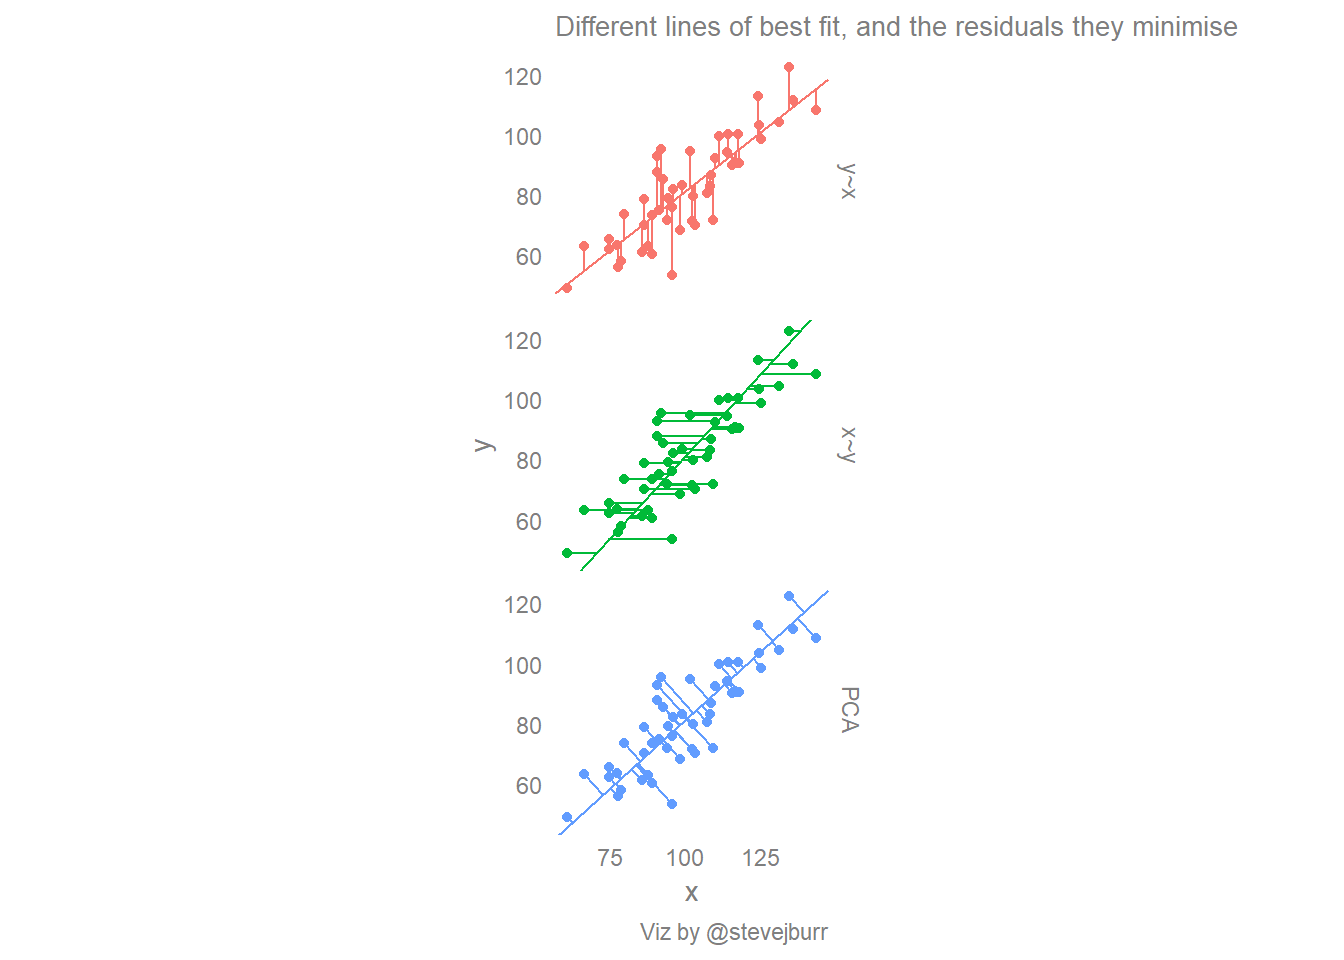
\includegraphics{2018-10-25-replicating-flowingdata-population-charts-in-r_files/figure-latex/unnamed-chunk-15-1.png}

In the original, the fill is slightly transparent so that you can see
the top line, so let's make a small change to both the fill alpha values
and the line widths to do that:

\begin{Shaded}
\begin{Highlighting}[]
\NormalTok{chartData }\OperatorTok\StringTok{ }\KeywordTok{filter}\NormalTok{(Year}\OperatorTok{==}\DecValTok{2014}\NormalTok{) }\OperatorTok
\StringTok{  }\KeywordTok{ggplot}\NormalTok{() }\OperatorTok{+}
\StringTok{  }\KeywordTok{geom_ribbon}\NormalTok{(}\KeywordTok{aes}\NormalTok{(}\DataTypeTok{x=}\StringTok{`}\DataTypeTok{Age Code}\StringTok{`}\NormalTok{,}\DataTypeTok{ymin=}\NormalTok{Lower,}\DataTypeTok{ymax=}\NormalTok{Upper,}\DataTypeTok{fill=}\NormalTok{UpperGender),}
              \DataTypeTok{alpha=}\FloatTok{0.8}\NormalTok{) }\OperatorTok{+}\StringTok{ }\CommentTok{#make fill slightly transparent}
\StringTok{  }\KeywordTok{geom_line}\NormalTok{(}\KeywordTok{aes}\NormalTok{(}\DataTypeTok{x=}\StringTok{`}\DataTypeTok{Age Code}\StringTok{`}\NormalTok{,}\DataTypeTok{y=}\NormalTok{Lower,}\DataTypeTok{colour=}\NormalTok{LowerGender),}\DataTypeTok{size=}\FloatTok{0.9}\NormalTok{,}\DataTypeTok{show.legend =} \OtherTok{FALSE}\NormalTok{) }\OperatorTok{+}\StringTok{ }
\StringTok{  }\KeywordTok{geom_line}\NormalTok{(}\KeywordTok{aes}\NormalTok{(}\DataTypeTok{x=}\StringTok{`}\DataTypeTok{Age Code}\StringTok{`}\NormalTok{,}\DataTypeTok{y=}\NormalTok{Upper,}\DataTypeTok{colour=}\NormalTok{UpperGender),}\DataTypeTok{size=}\FloatTok{0.9}\NormalTok{,}\DataTypeTok{show.legend =} \OtherTok{FALSE}\NormalTok{) }\OperatorTok{+}\StringTok{ }\CommentTok{#we don't need the line colours to have a legend}
\StringTok{  }\KeywordTok{scale_fill_manual}\NormalTok{(}\StringTok{""}\NormalTok{,}\CommentTok{#don't label the legend}
                    \DataTypeTok{breaks=}\KeywordTok{c}\NormalTok{(}\StringTok{"Male"}\NormalTok{,}\StringTok{"Female"}\NormalTok{), }\CommentTok{#choose the order to display in }
                    \DataTypeTok{labels=}\KeywordTok{c}\NormalTok{(}\StringTok{"More Men"}\NormalTok{,}\StringTok{"More Women"}\NormalTok{), }\CommentTok{#match the labelling used in the original}
                    \DataTypeTok{values=}\KeywordTok{c}\NormalTok{(women,men), }\CommentTok{#colours to use, in the order of the factor not displayed order}
                    \DataTypeTok{aesthetics =} \KeywordTok{c}\NormalTok{(}\StringTok{"colour"}\NormalTok{, }\StringTok{"fill"}\NormalTok{))}\OperatorTok{+}\StringTok{ }\CommentTok{#change both the line and fills together}
\StringTok{  }\KeywordTok{scale_y_continuous}\NormalTok{(}\StringTok{""}\NormalTok{, }\CommentTok{#the title for the axis}
                     \DataTypeTok{limits=}\KeywordTok{c}\NormalTok{(}\DecValTok{0}\NormalTok{,}\DecValTok{3000000}\NormalTok{), }\CommentTok{#set the top and bottom value}
                     \DataTypeTok{expand=}\KeywordTok{c}\NormalTok{(}\DecValTok{0}\NormalTok{,}\DecValTok{0}\NormalTok{), }\CommentTok{#don't expand beyond the specified limits}
                     \DataTypeTok{breaks=}\KeywordTok{c}\NormalTok{(}\DecValTok{0}\NormalTok{,}\DecValTok{500000}\NormalTok{,}\DecValTok{1000000}\NormalTok{,}\DecValTok{1500000}\NormalTok{,}\DecValTok{2000000}\NormalTok{,}\DecValTok{2500000}\NormalTok{,}\DecValTok{3000000}\NormalTok{), }\CommentTok{#specify what to put on the axis}
                     \DataTypeTok{labels=}\NormalTok{scales}\OperatorTok{::}\KeywordTok{comma_format}\NormalTok{(}\DataTypeTok{scale=}\FloatTok{0.001}\NormalTok{,}\DataTypeTok{suffix=}\StringTok{"k"}\NormalTok{)) }\OperatorTok{+}\StringTok{ }\CommentTok{# format the displayed numbers using the scales package}
\StringTok{  }\KeywordTok{scale_x_continuous}\NormalTok{(}\StringTok{"AGE"}\NormalTok{, }\CommentTok{#axis title}
                     \DataTypeTok{breaks=} \KeywordTok{c}\NormalTok{(}\DecValTok{0}\NormalTok{,}\DecValTok{10}\NormalTok{,}\DecValTok{20}\NormalTok{,}\DecValTok{30}\NormalTok{,}\DecValTok{40}\NormalTok{,}\DecValTok{50}\NormalTok{,}\DecValTok{60}\NormalTok{,}\DecValTok{70}\NormalTok{,}\DecValTok{80}\NormalTok{,}\DecValTok{90}\NormalTok{,}\DecValTok{100}\NormalTok{),}
                     \DataTypeTok{labels=}\KeywordTok{c}\NormalTok{(}\StringTok{"0"}\NormalTok{,}\StringTok{"10"}\NormalTok{,}\StringTok{"20"}\NormalTok{,}\StringTok{"30"}\NormalTok{,}\StringTok{"40"}\NormalTok{,}\StringTok{"50"}\NormalTok{,}\StringTok{"60"}\NormalTok{,}\StringTok{"70"}\NormalTok{,}\StringTok{"80"}\NormalTok{,}\StringTok{"90"}\NormalTok{,}\StringTok{"100+"}\NormalTok{)) }\OperatorTok{+}
\StringTok{  }\KeywordTok{labs}\NormalTok{(}\DataTypeTok{subtitle=}\StringTok{"POPULATION"}\NormalTok{)}\OperatorTok{+}
\StringTok{  }\KeywordTok{theme_minimal}\NormalTok{() }\OperatorTok{+}\StringTok{ }\CommentTok{#apply my prefered theme which is close to what Nathan used}
\StringTok{  }\KeywordTok{theme}\NormalTok{(}\DataTypeTok{text=}\KeywordTok{element_text}\NormalTok{(}\DataTypeTok{colour=}\StringTok{"black"}\NormalTok{), }\CommentTok{#all text is black}
        \DataTypeTok{plot.subtitle=}\KeywordTok{element_text}\NormalTok{(}\DataTypeTok{size=}\DecValTok{9}\NormalTok{),}
        \DataTypeTok{axis.text =} \KeywordTok{element_text}\NormalTok{(}\DataTypeTok{colour=}\StringTok{"black"}\NormalTok{), }\CommentTok{#make sure labels are black also}
        \DataTypeTok{axis.title.x=}\KeywordTok{element_text}\NormalTok{(}\DataTypeTok{hjust=}\DecValTok{0}\NormalTok{,}\DataTypeTok{angle=}\DecValTok{0}\NormalTok{,}\DataTypeTok{size=}\DecValTok{9}\NormalTok{),}
        \DataTypeTok{panel.grid.minor.x=}\KeywordTok{element_blank}\NormalTok{(), }\CommentTok{#turn off minor gridlines}
        \DataTypeTok{panel.grid.minor.y=}\KeywordTok{element_blank}\NormalTok{(), }\CommentTok{#turn off minor gridlines}
        \DataTypeTok{legend.position =} \KeywordTok{c}\NormalTok{(}\FloatTok{0.2}\NormalTok{,}\FloatTok{0.92}\NormalTok{), }\CommentTok{#position legend over the plot}
        \DataTypeTok{legend.text =} \KeywordTok{element_text}\NormalTok{(}\DataTypeTok{face=}\StringTok{"italic"}\NormalTok{) }\CommentTok{#make italic}
\NormalTok{        ) ->}\StringTok{ }\NormalTok{p}

\CommentTok{#turn the plot into a gtable object}
\NormalTok{g <-}\StringTok{ }\KeywordTok{ggplotGrob}\NormalTok{(p)}
\CommentTok{#adjust the position of the subtitle}
\NormalTok{g}\OperatorTok{$}\NormalTok{layout}\OperatorTok{$}\NormalTok{l[g}\OperatorTok{$}\NormalTok{layout}\OperatorTok{$}\NormalTok{name }\OperatorTok{==}\StringTok{ "subtitle"}\NormalTok{] <-}\StringTok{ }\DecValTok{1}
\CommentTok{#draw the new plot}
\NormalTok{grid}\OperatorTok{::}\KeywordTok{grid.draw}\NormalTok{(g)}
\end{Highlighting}
\end{Shaded}

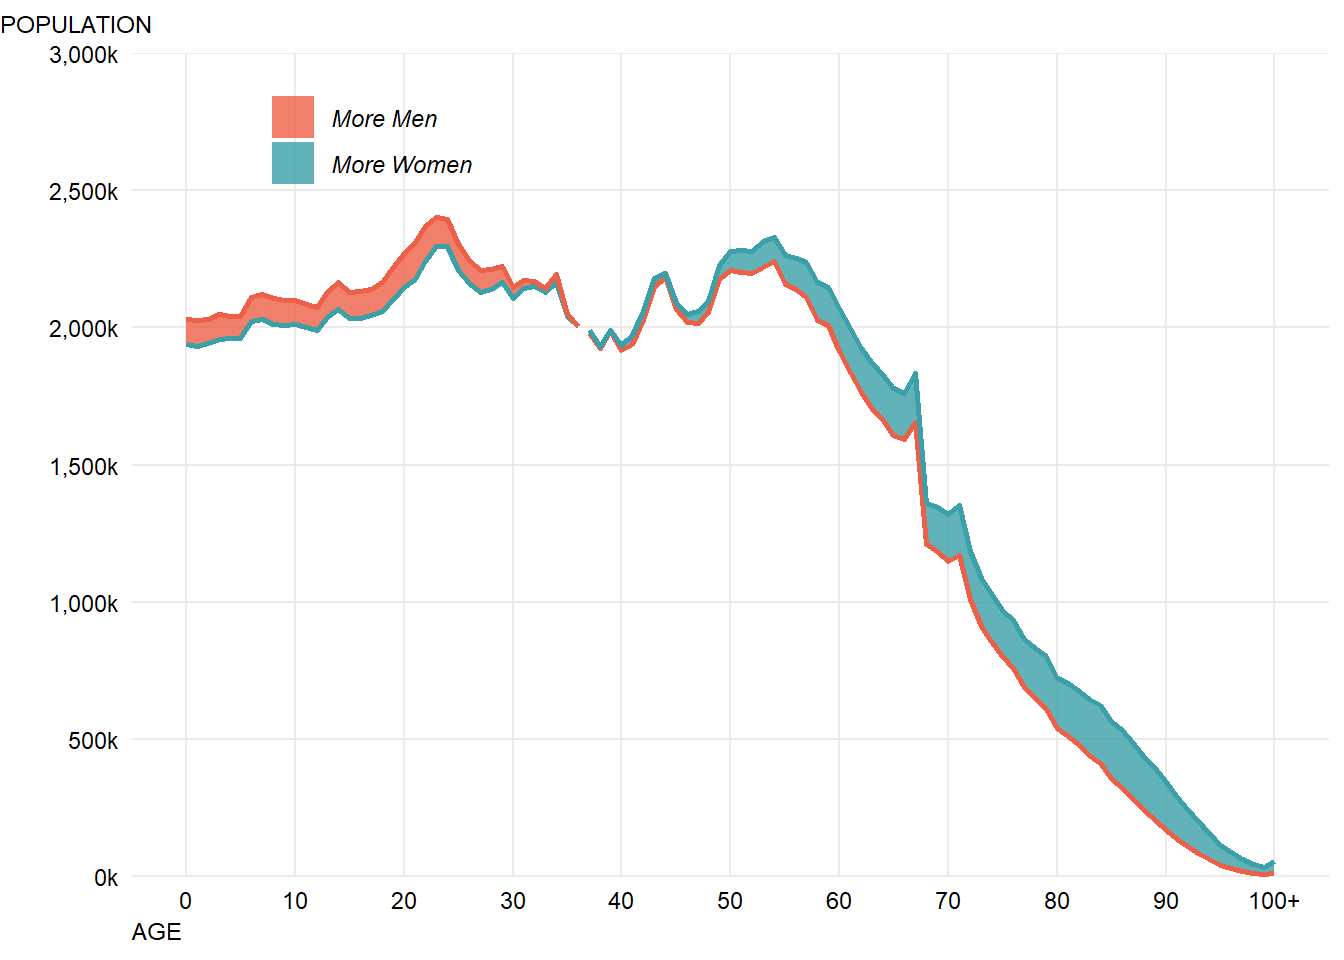
\includegraphics{2018-10-25-replicating-flowingdata-population-charts-in-r_files/figure-latex/unnamed-chunk-16-1.png}

This looks pretty close now, having a quick scan through Google Fonts,
it looks like ``Roboto Mono'' is somewhat similar to the font use so
I'll go with that and apply it using the showtext package:

\begin{Shaded}
\begin{Highlighting}[]
\KeywordTok{library}\NormalTok{(showtext)}
\KeywordTok{font_add_google}\NormalTok{(}\StringTok{"Roboto Mono"}\NormalTok{, }\StringTok{"roboto"}\NormalTok{)}



\KeywordTok{showtext_auto}\NormalTok{()}

\NormalTok{chartData }\OperatorTok\StringTok{ }\KeywordTok{filter}\NormalTok{(Year}\OperatorTok{==}\DecValTok{2014}\NormalTok{) }\OperatorTok
\StringTok{  }\KeywordTok{ggplot}\NormalTok{() }\OperatorTok{+}
\StringTok{  }\KeywordTok{geom_ribbon}\NormalTok{(}\KeywordTok{aes}\NormalTok{(}\DataTypeTok{x=}\StringTok{`}\DataTypeTok{Age Code}\StringTok{`}\NormalTok{,}\DataTypeTok{ymin=}\NormalTok{Lower,}\DataTypeTok{ymax=}\NormalTok{Upper,}\DataTypeTok{fill=}\NormalTok{UpperGender),}
              \DataTypeTok{alpha=}\FloatTok{0.8}\NormalTok{) }\OperatorTok{+}\StringTok{ }\CommentTok{#make fill slightly transparent}
\StringTok{  }\KeywordTok{geom_line}\NormalTok{(}\KeywordTok{aes}\NormalTok{(}\DataTypeTok{x=}\StringTok{`}\DataTypeTok{Age Code}\StringTok{`}\NormalTok{,}\DataTypeTok{y=}\NormalTok{Lower,}\DataTypeTok{colour=}\NormalTok{LowerGender),}\DataTypeTok{size=}\FloatTok{0.9}\NormalTok{,}\DataTypeTok{show.legend =} \OtherTok{FALSE}\NormalTok{) }\OperatorTok{+}\StringTok{ }
\StringTok{  }\KeywordTok{geom_line}\NormalTok{(}\KeywordTok{aes}\NormalTok{(}\DataTypeTok{x=}\StringTok{`}\DataTypeTok{Age Code}\StringTok{`}\NormalTok{,}\DataTypeTok{y=}\NormalTok{Upper,}\DataTypeTok{colour=}\NormalTok{UpperGender),}\DataTypeTok{size=}\FloatTok{0.9}\NormalTok{,}\DataTypeTok{show.legend =} \OtherTok{FALSE}\NormalTok{) }\OperatorTok{+}\StringTok{ }\CommentTok{#we don't need the line colours to have a legend}
\StringTok{  }\KeywordTok{scale_fill_manual}\NormalTok{(}\StringTok{""}\NormalTok{,}\CommentTok{#don't label the legend}
                    \DataTypeTok{breaks=}\KeywordTok{c}\NormalTok{(}\StringTok{"Male"}\NormalTok{,}\StringTok{"Female"}\NormalTok{), }\CommentTok{#choose the order to display in }
                    \DataTypeTok{labels=}\KeywordTok{c}\NormalTok{(}\StringTok{"More Men"}\NormalTok{,}\StringTok{"More Women"}\NormalTok{), }\CommentTok{#match the labelling used in the original}
                    \DataTypeTok{values=}\KeywordTok{c}\NormalTok{(women,men), }\CommentTok{#colours to use, in the order of the factor not displayed order}
                    \DataTypeTok{aesthetics =} \KeywordTok{c}\NormalTok{(}\StringTok{"colour"}\NormalTok{, }\StringTok{"fill"}\NormalTok{))}\OperatorTok{+}\StringTok{ }\CommentTok{#change both the line and fills together}
\StringTok{  }\KeywordTok{scale_y_continuous}\NormalTok{(}\StringTok{""}\NormalTok{, }\CommentTok{#the title for the axis}
                     \DataTypeTok{limits=}\KeywordTok{c}\NormalTok{(}\DecValTok{0}\NormalTok{,}\DecValTok{3000000}\NormalTok{), }\CommentTok{#set the top and bottom value}
                     \DataTypeTok{expand=}\KeywordTok{c}\NormalTok{(}\DecValTok{0}\NormalTok{,}\DecValTok{0}\NormalTok{), }\CommentTok{#don't expand beyond the specified limits}
                     \DataTypeTok{breaks=}\KeywordTok{c}\NormalTok{(}\DecValTok{0}\NormalTok{,}\DecValTok{500000}\NormalTok{,}\DecValTok{1000000}\NormalTok{,}\DecValTok{1500000}\NormalTok{,}\DecValTok{2000000}\NormalTok{,}\DecValTok{2500000}\NormalTok{,}\DecValTok{3000000}\NormalTok{), }\CommentTok{#specify what to put on the axis}
                     \DataTypeTok{labels=}\NormalTok{scales}\OperatorTok{::}\KeywordTok{comma_format}\NormalTok{(}\DataTypeTok{scale=}\FloatTok{0.001}\NormalTok{,}\DataTypeTok{suffix=}\StringTok{"k"}\NormalTok{)) }\OperatorTok{+}\StringTok{ }\CommentTok{# format the displayed numbers using the scales package}
\StringTok{  }\KeywordTok{scale_x_continuous}\NormalTok{(}\StringTok{"AGE"}\NormalTok{, }\CommentTok{#axis title}
                     \DataTypeTok{breaks=} \KeywordTok{c}\NormalTok{(}\DecValTok{0}\NormalTok{,}\DecValTok{10}\NormalTok{,}\DecValTok{20}\NormalTok{,}\DecValTok{30}\NormalTok{,}\DecValTok{40}\NormalTok{,}\DecValTok{50}\NormalTok{,}\DecValTok{60}\NormalTok{,}\DecValTok{70}\NormalTok{,}\DecValTok{80}\NormalTok{,}\DecValTok{90}\NormalTok{,}\DecValTok{100}\NormalTok{),}
                     \DataTypeTok{labels=}\KeywordTok{c}\NormalTok{(}\StringTok{"0"}\NormalTok{,}\StringTok{"10"}\NormalTok{,}\StringTok{"20"}\NormalTok{,}\StringTok{"30"}\NormalTok{,}\StringTok{"40"}\NormalTok{,}\StringTok{"50"}\NormalTok{,}\StringTok{"60"}\NormalTok{,}\StringTok{"70"}\NormalTok{,}\StringTok{"80"}\NormalTok{,}\StringTok{"90"}\NormalTok{,}\StringTok{"100+"}\NormalTok{)) }\OperatorTok{+}
\StringTok{  }\KeywordTok{labs}\NormalTok{(}\DataTypeTok{subtitle=}\StringTok{"POPULATION"}\NormalTok{)}\OperatorTok{+}
\StringTok{  }\KeywordTok{theme_minimal}\NormalTok{() }\OperatorTok{+}\StringTok{ }\CommentTok{#apply my prefered theme which is close to what Nathan used}
\StringTok{  }\KeywordTok{theme}\NormalTok{(}\DataTypeTok{text=}\KeywordTok{element_text}\NormalTok{(}\DataTypeTok{colour=}\StringTok{"black"}\NormalTok{,}\DataTypeTok{family=}\StringTok{"roboto"}\NormalTok{), }\CommentTok{#all text is black}
        \DataTypeTok{plot.subtitle=}\KeywordTok{element_text}\NormalTok{(}\DataTypeTok{size=}\DecValTok{9}\NormalTok{),}
        \DataTypeTok{axis.text =} \KeywordTok{element_text}\NormalTok{(}\DataTypeTok{colour=}\StringTok{"black"}\NormalTok{), }\CommentTok{#make sure labels are black also}
        \DataTypeTok{axis.title.x=}\KeywordTok{element_text}\NormalTok{(}\DataTypeTok{hjust=}\DecValTok{0}\NormalTok{,}\DataTypeTok{angle=}\DecValTok{0}\NormalTok{,}\DataTypeTok{size=}\DecValTok{9}\NormalTok{),}
        \DataTypeTok{panel.grid.minor.x=}\KeywordTok{element_blank}\NormalTok{(), }\CommentTok{#turn off minor gridlines}
        \DataTypeTok{panel.grid.minor.y=}\KeywordTok{element_blank}\NormalTok{(), }\CommentTok{#turn off minor gridlines}
        \DataTypeTok{legend.position =} \KeywordTok{c}\NormalTok{(}\FloatTok{0.2}\NormalTok{,}\FloatTok{0.92}\NormalTok{), }\CommentTok{#position legend over the plot}
        \DataTypeTok{legend.text =} \KeywordTok{element_text}\NormalTok{(}\DataTypeTok{face=}\StringTok{"italic"}\NormalTok{) }\CommentTok{#make italic}
\NormalTok{        ) }
\end{Highlighting}
\end{Shaded}

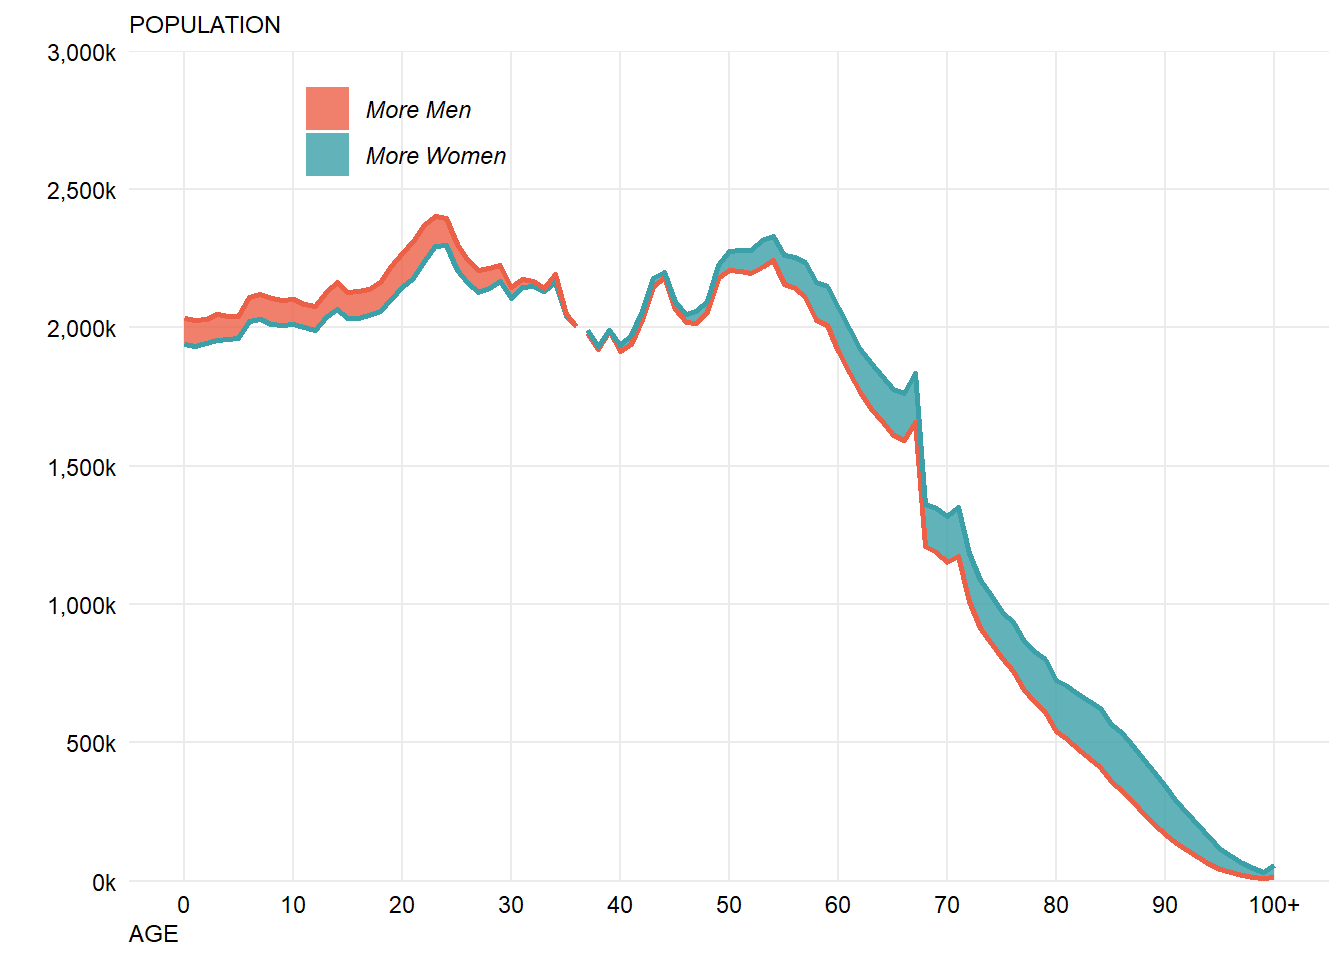
\includegraphics{2018-10-25-replicating-flowingdata-population-charts-in-r_files/figure-latex/unnamed-chunk-17-1.png}
Unfortunately this way of specifying fonts doesn't seem to play nicely
with my solution to left aligning the title (at least within an R
Markdown document). An alternative is to just manually tweak the hjust
value until the positioning looks right in this case (this is not
transferable to different lenght titles, but that doesn't matter for
this example).

\begin{Shaded}
\begin{Highlighting}[]
\KeywordTok{showtext_auto}\NormalTok{()}

\NormalTok{chartData }\OperatorTok\StringTok{ }\KeywordTok{filter}\NormalTok{(Year}\OperatorTok{==}\DecValTok{2014}\NormalTok{) }\OperatorTok
\StringTok{  }\KeywordTok{ggplot}\NormalTok{() }\OperatorTok{+}
\StringTok{  }\KeywordTok{geom_ribbon}\NormalTok{(}\KeywordTok{aes}\NormalTok{(}\DataTypeTok{x=}\StringTok{`}\DataTypeTok{Age Code}\StringTok{`}\NormalTok{,}\DataTypeTok{ymin=}\NormalTok{Lower,}\DataTypeTok{ymax=}\NormalTok{Upper,}\DataTypeTok{fill=}\NormalTok{UpperGender),}
              \DataTypeTok{alpha=}\FloatTok{0.8}\NormalTok{) }\OperatorTok{+}\StringTok{ }\CommentTok{#make fill slightly transparent}
\StringTok{  }\KeywordTok{geom_line}\NormalTok{(}\KeywordTok{aes}\NormalTok{(}\DataTypeTok{x=}\StringTok{`}\DataTypeTok{Age Code}\StringTok{`}\NormalTok{,}\DataTypeTok{y=}\NormalTok{Lower,}\DataTypeTok{colour=}\NormalTok{LowerGender),}\DataTypeTok{size=}\FloatTok{0.9}\NormalTok{,}\DataTypeTok{show.legend =} \OtherTok{FALSE}\NormalTok{) }\OperatorTok{+}\StringTok{ }
\StringTok{  }\KeywordTok{geom_line}\NormalTok{(}\KeywordTok{aes}\NormalTok{(}\DataTypeTok{x=}\StringTok{`}\DataTypeTok{Age Code}\StringTok{`}\NormalTok{,}\DataTypeTok{y=}\NormalTok{Upper,}\DataTypeTok{colour=}\NormalTok{UpperGender),}\DataTypeTok{size=}\FloatTok{0.9}\NormalTok{,}\DataTypeTok{show.legend =} \OtherTok{FALSE}\NormalTok{) }\OperatorTok{+}\StringTok{ }\CommentTok{#we don't need the line colours to have a legend}
\StringTok{  }\KeywordTok{scale_fill_manual}\NormalTok{(}\StringTok{""}\NormalTok{,}\CommentTok{#don't label the legend}
                    \DataTypeTok{breaks=}\KeywordTok{c}\NormalTok{(}\StringTok{"Male"}\NormalTok{,}\StringTok{"Female"}\NormalTok{), }\CommentTok{#choose the order to display in }
                    \DataTypeTok{labels=}\KeywordTok{c}\NormalTok{(}\StringTok{"More Men"}\NormalTok{,}\StringTok{"More Women"}\NormalTok{), }\CommentTok{#match the labelling used in the original}
                    \DataTypeTok{values=}\KeywordTok{c}\NormalTok{(women,men), }\CommentTok{#colours to use, in the order of the factor not displayed order}
                    \DataTypeTok{aesthetics =} \KeywordTok{c}\NormalTok{(}\StringTok{"colour"}\NormalTok{, }\StringTok{"fill"}\NormalTok{))}\OperatorTok{+}\StringTok{ }\CommentTok{#change both the line and fills together}
\StringTok{  }\KeywordTok{scale_y_continuous}\NormalTok{(}\StringTok{""}\NormalTok{, }\CommentTok{#the title for the axis}
                     \DataTypeTok{limits=}\KeywordTok{c}\NormalTok{(}\DecValTok{0}\NormalTok{,}\DecValTok{3000000}\NormalTok{), }\CommentTok{#set the top and bottom value}
                     \DataTypeTok{expand=}\KeywordTok{c}\NormalTok{(}\DecValTok{0}\NormalTok{,}\DecValTok{0}\NormalTok{), }\CommentTok{#don't expand beyond the specified limits}
                     \DataTypeTok{breaks=}\KeywordTok{c}\NormalTok{(}\DecValTok{0}\NormalTok{,}\DecValTok{500000}\NormalTok{,}\DecValTok{1000000}\NormalTok{,}\DecValTok{1500000}\NormalTok{,}\DecValTok{2000000}\NormalTok{,}\DecValTok{2500000}\NormalTok{,}\DecValTok{3000000}\NormalTok{), }\CommentTok{#specify what to put on the axis}
                     \DataTypeTok{labels=}\NormalTok{scales}\OperatorTok{::}\KeywordTok{comma_format}\NormalTok{(}\DataTypeTok{scale=}\FloatTok{0.001}\NormalTok{,}\DataTypeTok{suffix=}\StringTok{"k"}\NormalTok{)) }\OperatorTok{+}\StringTok{ }\CommentTok{# format the displayed numbers using the scales package}
\StringTok{  }\KeywordTok{scale_x_continuous}\NormalTok{(}\StringTok{"AGE"}\NormalTok{, }\CommentTok{#axis title}
                     \DataTypeTok{breaks=} \KeywordTok{c}\NormalTok{(}\DecValTok{0}\NormalTok{,}\DecValTok{10}\NormalTok{,}\DecValTok{20}\NormalTok{,}\DecValTok{30}\NormalTok{,}\DecValTok{40}\NormalTok{,}\DecValTok{50}\NormalTok{,}\DecValTok{60}\NormalTok{,}\DecValTok{70}\NormalTok{,}\DecValTok{80}\NormalTok{,}\DecValTok{90}\NormalTok{,}\DecValTok{100}\NormalTok{),}
                     \DataTypeTok{labels=}\KeywordTok{c}\NormalTok{(}\StringTok{"0"}\NormalTok{,}\StringTok{"10"}\NormalTok{,}\StringTok{"20"}\NormalTok{,}\StringTok{"30"}\NormalTok{,}\StringTok{"40"}\NormalTok{,}\StringTok{"50"}\NormalTok{,}\StringTok{"60"}\NormalTok{,}\StringTok{"70"}\NormalTok{,}\StringTok{"80"}\NormalTok{,}\StringTok{"90"}\NormalTok{,}\StringTok{"100+"}\NormalTok{)) }\OperatorTok{+}
\StringTok{  }\KeywordTok{labs}\NormalTok{(}\DataTypeTok{subtitle=}\StringTok{"POPULATION"}\NormalTok{)}\OperatorTok{+}
\StringTok{  }\KeywordTok{theme_minimal}\NormalTok{() }\OperatorTok{+}\StringTok{ }\CommentTok{#apply my prefered theme which is close to what Nathan used}
\StringTok{  }\KeywordTok{theme}\NormalTok{(}\DataTypeTok{text=}\KeywordTok{element_text}\NormalTok{(}\DataTypeTok{colour=}\StringTok{"black"}\NormalTok{,}\DataTypeTok{family=}\StringTok{"roboto"}\NormalTok{), }\CommentTok{#all text is black}
        \DataTypeTok{plot.subtitle=}\KeywordTok{element_text}\NormalTok{(}\DataTypeTok{size=}\DecValTok{9}\NormalTok{,}\DataTypeTok{hjust=}\OperatorTok{-}\FloatTok{0.085}\NormalTok{), }\CommentTok{# manually tweak subtitle position}
        \DataTypeTok{axis.text =} \KeywordTok{element_text}\NormalTok{(}\DataTypeTok{colour=}\StringTok{"black"}\NormalTok{), }\CommentTok{#make sure labels are black also}
        \DataTypeTok{axis.title.x=}\KeywordTok{element_text}\NormalTok{(}\DataTypeTok{hjust=}\DecValTok{0}\NormalTok{,}\DataTypeTok{angle=}\DecValTok{0}\NormalTok{,}\DataTypeTok{size=}\DecValTok{9}\NormalTok{),}
        \DataTypeTok{panel.grid.minor.x=}\KeywordTok{element_blank}\NormalTok{(), }\CommentTok{#turn off minor gridlines}
        \DataTypeTok{panel.grid.minor.y=}\KeywordTok{element_blank}\NormalTok{(), }\CommentTok{#turn off minor gridlines}
        \DataTypeTok{legend.position =} \KeywordTok{c}\NormalTok{(}\FloatTok{0.2}\NormalTok{,}\FloatTok{0.92}\NormalTok{), }\CommentTok{#position legend over the plot}
        \DataTypeTok{legend.text =} \KeywordTok{element_text}\NormalTok{(}\DataTypeTok{face=}\StringTok{"italic"}\NormalTok{) }\CommentTok{#make italic}
\NormalTok{        ) }
\end{Highlighting}
\end{Shaded}

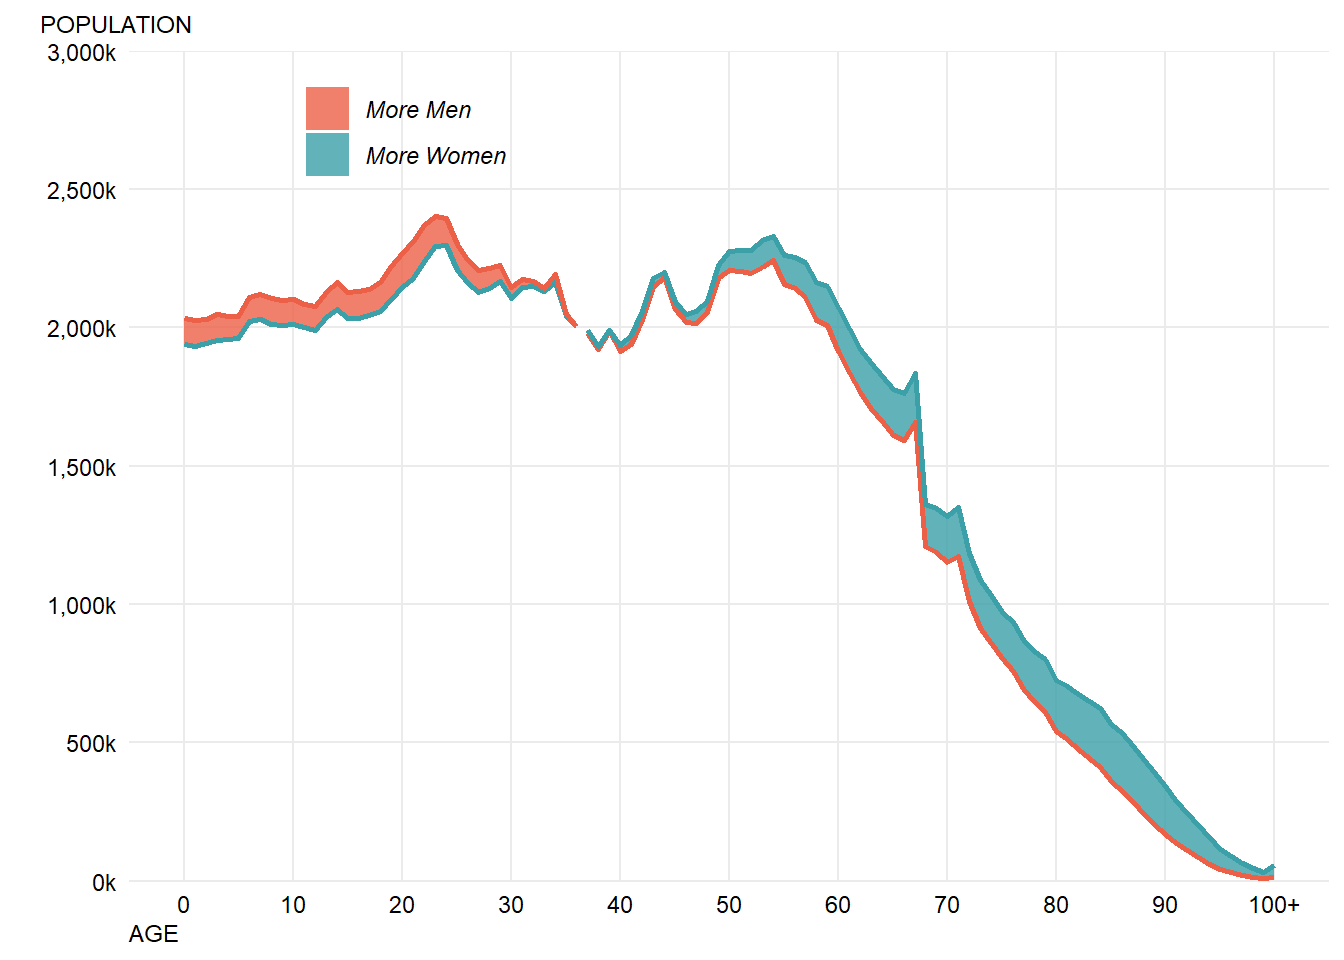
\includegraphics{2018-10-25-replicating-flowingdata-population-charts-in-r_files/figure-latex/unnamed-chunk-18-1.png}

There's one odd looking element, there's a gap in the plot where the
lines should cross over. One slightly hacky solution is to duplicate the
records where the cross over occurs:

\begin{Shaded}
\begin{Highlighting}[]
\NormalTok{chartData }\OperatorTok\StringTok{ }\KeywordTok{arrange}\NormalTok{(Year, }\StringTok{`}\DataTypeTok{Age Code}\StringTok{`}\NormalTok{) }\OperatorTok
\StringTok{  }\KeywordTok{filter}\NormalTok{(UpperGender}\OperatorTok{!=}\KeywordTok{lag}\NormalTok{(UpperGender) }\OperatorTok{&}\StringTok{`}\DataTypeTok{Age Code}\StringTok{`} \OperatorTok{>}\StringTok{ }\DecValTok{0}\NormalTok{) ->}\StringTok{ }\NormalTok{crossOvers}

\NormalTok{crossOvers }\OperatorTok\StringTok{ }\KeywordTok{mutate}\NormalTok{(}\DataTypeTok{UpperGender=}\KeywordTok{if_else}\NormalTok{(UpperGender}\OperatorTok{==}\StringTok{"Male"}\NormalTok{,}\StringTok{"Female"}\NormalTok{,}\StringTok{"Male"}\NormalTok{),}
                      \DataTypeTok{LowerGender=}\KeywordTok{if_else}\NormalTok{(LowerGender}\OperatorTok{==}\StringTok{"Male"}\NormalTok{,}\StringTok{"Female"}\NormalTok{,}\StringTok{"Male"}\NormalTok{)) ->}\StringTok{ }\NormalTok{crossOvers}

\NormalTok{chartData }\OperatorTok\StringTok{ }\KeywordTok{rbind}\NormalTok{(crossOvers) ->}\StringTok{ }\NormalTok{chartData2}
\end{Highlighting}
\end{Shaded}

Another solution might be to explictly draw two ribbons for each year
and not rely on ggplot2 to fill in the gaps.

The hacky solution broadly looks like it works:

\begin{Shaded}
\begin{Highlighting}[]
\NormalTok{chartData2 }\OperatorTok\StringTok{ }\KeywordTok{filter}\NormalTok{(Year}\OperatorTok{==}\DecValTok{2014}\NormalTok{) }\OperatorTok
\StringTok{  }\KeywordTok{ggplot}\NormalTok{() }\OperatorTok{+}
\StringTok{  }\KeywordTok{geom_ribbon}\NormalTok{(}\KeywordTok{aes}\NormalTok{(}\DataTypeTok{x=}\StringTok{`}\DataTypeTok{Age Code}\StringTok{`}\NormalTok{,}\DataTypeTok{ymin=}\NormalTok{Lower,}\DataTypeTok{ymax=}\NormalTok{Upper,}\DataTypeTok{fill=}\NormalTok{UpperGender),}
              \DataTypeTok{alpha=}\FloatTok{0.8}\NormalTok{) }\OperatorTok{+}\StringTok{ }\CommentTok{#make fill slightly transparent}
\StringTok{  }\KeywordTok{geom_line}\NormalTok{(}\KeywordTok{aes}\NormalTok{(}\DataTypeTok{x=}\StringTok{`}\DataTypeTok{Age Code}\StringTok{`}\NormalTok{,}\DataTypeTok{y=}\NormalTok{Lower,}\DataTypeTok{colour=}\NormalTok{LowerGender),}\DataTypeTok{size=}\FloatTok{0.9}\NormalTok{,}\DataTypeTok{show.legend =} \OtherTok{FALSE}\NormalTok{) }\OperatorTok{+}\StringTok{ }
\StringTok{  }\KeywordTok{geom_line}\NormalTok{(}\KeywordTok{aes}\NormalTok{(}\DataTypeTok{x=}\StringTok{`}\DataTypeTok{Age Code}\StringTok{`}\NormalTok{,}\DataTypeTok{y=}\NormalTok{Upper,}\DataTypeTok{colour=}\NormalTok{UpperGender),}\DataTypeTok{size=}\FloatTok{0.9}\NormalTok{,}\DataTypeTok{show.legend =} \OtherTok{FALSE}\NormalTok{) }\OperatorTok{+}\StringTok{ }\CommentTok{#we don't need the line colours to have a legend}
\StringTok{  }\KeywordTok{scale_fill_manual}\NormalTok{(}\StringTok{""}\NormalTok{,}\CommentTok{#don't label the legend}
                    \DataTypeTok{breaks=}\KeywordTok{c}\NormalTok{(}\StringTok{"Male"}\NormalTok{,}\StringTok{"Female"}\NormalTok{), }\CommentTok{#choose the order to display in }
                    \DataTypeTok{labels=}\KeywordTok{c}\NormalTok{(}\StringTok{"More Men"}\NormalTok{,}\StringTok{"More Women"}\NormalTok{), }\CommentTok{#match the labelling used in the original}
                    \DataTypeTok{values=}\KeywordTok{c}\NormalTok{(women,men), }\CommentTok{#colours to use, in the order of the factor not displayed order}
                    \DataTypeTok{aesthetics =} \KeywordTok{c}\NormalTok{(}\StringTok{"colour"}\NormalTok{, }\StringTok{"fill"}\NormalTok{))}\OperatorTok{+}\StringTok{ }\CommentTok{#change both the line and fills together}
\StringTok{  }\KeywordTok{scale_y_continuous}\NormalTok{(}\StringTok{""}\NormalTok{, }\CommentTok{#the title for the axis}
                     \DataTypeTok{limits=}\KeywordTok{c}\NormalTok{(}\DecValTok{0}\NormalTok{,}\DecValTok{3000000}\NormalTok{), }\CommentTok{#set the top and bottom value}
                     \DataTypeTok{expand=}\KeywordTok{c}\NormalTok{(}\DecValTok{0}\NormalTok{,}\DecValTok{0}\NormalTok{), }\CommentTok{#don't expand beyond the specified limits}
                     \DataTypeTok{breaks=}\KeywordTok{c}\NormalTok{(}\DecValTok{0}\NormalTok{,}\DecValTok{500000}\NormalTok{,}\DecValTok{1000000}\NormalTok{,}\DecValTok{1500000}\NormalTok{,}\DecValTok{2000000}\NormalTok{,}\DecValTok{2500000}\NormalTok{,}\DecValTok{3000000}\NormalTok{), }\CommentTok{#specify what to put on the axis}
                     \DataTypeTok{labels=}\NormalTok{scales}\OperatorTok{::}\KeywordTok{comma_format}\NormalTok{(}\DataTypeTok{scale=}\FloatTok{0.001}\NormalTok{,}\DataTypeTok{suffix=}\StringTok{"k"}\NormalTok{)) }\OperatorTok{+}\StringTok{ }\CommentTok{# format the displayed numbers using the scales package}
\StringTok{  }\KeywordTok{scale_x_continuous}\NormalTok{(}\StringTok{"AGE"}\NormalTok{, }\CommentTok{#axis title}
                     \DataTypeTok{breaks=} \KeywordTok{c}\NormalTok{(}\DecValTok{0}\NormalTok{,}\DecValTok{10}\NormalTok{,}\DecValTok{20}\NormalTok{,}\DecValTok{30}\NormalTok{,}\DecValTok{40}\NormalTok{,}\DecValTok{50}\NormalTok{,}\DecValTok{60}\NormalTok{,}\DecValTok{70}\NormalTok{,}\DecValTok{80}\NormalTok{,}\DecValTok{90}\NormalTok{,}\DecValTok{100}\NormalTok{),}
                     \DataTypeTok{labels=}\KeywordTok{c}\NormalTok{(}\StringTok{"0"}\NormalTok{,}\StringTok{"10"}\NormalTok{,}\StringTok{"20"}\NormalTok{,}\StringTok{"30"}\NormalTok{,}\StringTok{"40"}\NormalTok{,}\StringTok{"50"}\NormalTok{,}\StringTok{"60"}\NormalTok{,}\StringTok{"70"}\NormalTok{,}\StringTok{"80"}\NormalTok{,}\StringTok{"90"}\NormalTok{,}\StringTok{"100+"}\NormalTok{)) }\OperatorTok{+}
\StringTok{  }\KeywordTok{labs}\NormalTok{(}\DataTypeTok{subtitle=}\StringTok{"POPULATION"}\NormalTok{)}\OperatorTok{+}
\StringTok{  }\KeywordTok{theme_minimal}\NormalTok{() }\OperatorTok{+}\StringTok{ }\CommentTok{#apply my prefered theme which is close to what Nathan used}
\StringTok{  }\KeywordTok{theme}\NormalTok{(}\DataTypeTok{text=}\KeywordTok{element_text}\NormalTok{(}\DataTypeTok{colour=}\StringTok{"black"}\NormalTok{,}\DataTypeTok{family=}\StringTok{"roboto"}\NormalTok{), }\CommentTok{#all text is black}
        \DataTypeTok{plot.subtitle=}\KeywordTok{element_text}\NormalTok{(}\DataTypeTok{size=}\DecValTok{9}\NormalTok{,}\DataTypeTok{hjust=}\OperatorTok{-}\FloatTok{0.085}\NormalTok{), }\CommentTok{# manually tweak subtitle position}
        \DataTypeTok{axis.text =} \KeywordTok{element_text}\NormalTok{(}\DataTypeTok{colour=}\StringTok{"black"}\NormalTok{), }\CommentTok{#make sure labels are black also}
        \DataTypeTok{axis.title.x=}\KeywordTok{element_text}\NormalTok{(}\DataTypeTok{hjust=}\DecValTok{0}\NormalTok{,}\DataTypeTok{angle=}\DecValTok{0}\NormalTok{,}\DataTypeTok{size=}\DecValTok{9}\NormalTok{),}
        \DataTypeTok{panel.grid.minor.x=}\KeywordTok{element_blank}\NormalTok{(), }\CommentTok{#turn off minor gridlines}
        \DataTypeTok{panel.grid.minor.y=}\KeywordTok{element_blank}\NormalTok{(), }\CommentTok{#turn off minor gridlines}
        \DataTypeTok{legend.position =} \KeywordTok{c}\NormalTok{(}\FloatTok{0.2}\NormalTok{,}\FloatTok{0.92}\NormalTok{), }\CommentTok{#position legend over the plot}
        \DataTypeTok{legend.text =} \KeywordTok{element_text}\NormalTok{(}\DataTypeTok{face=}\StringTok{"italic"}\NormalTok{) }\CommentTok{#make italic}
\NormalTok{        ) }
\end{Highlighting}
\end{Shaded}

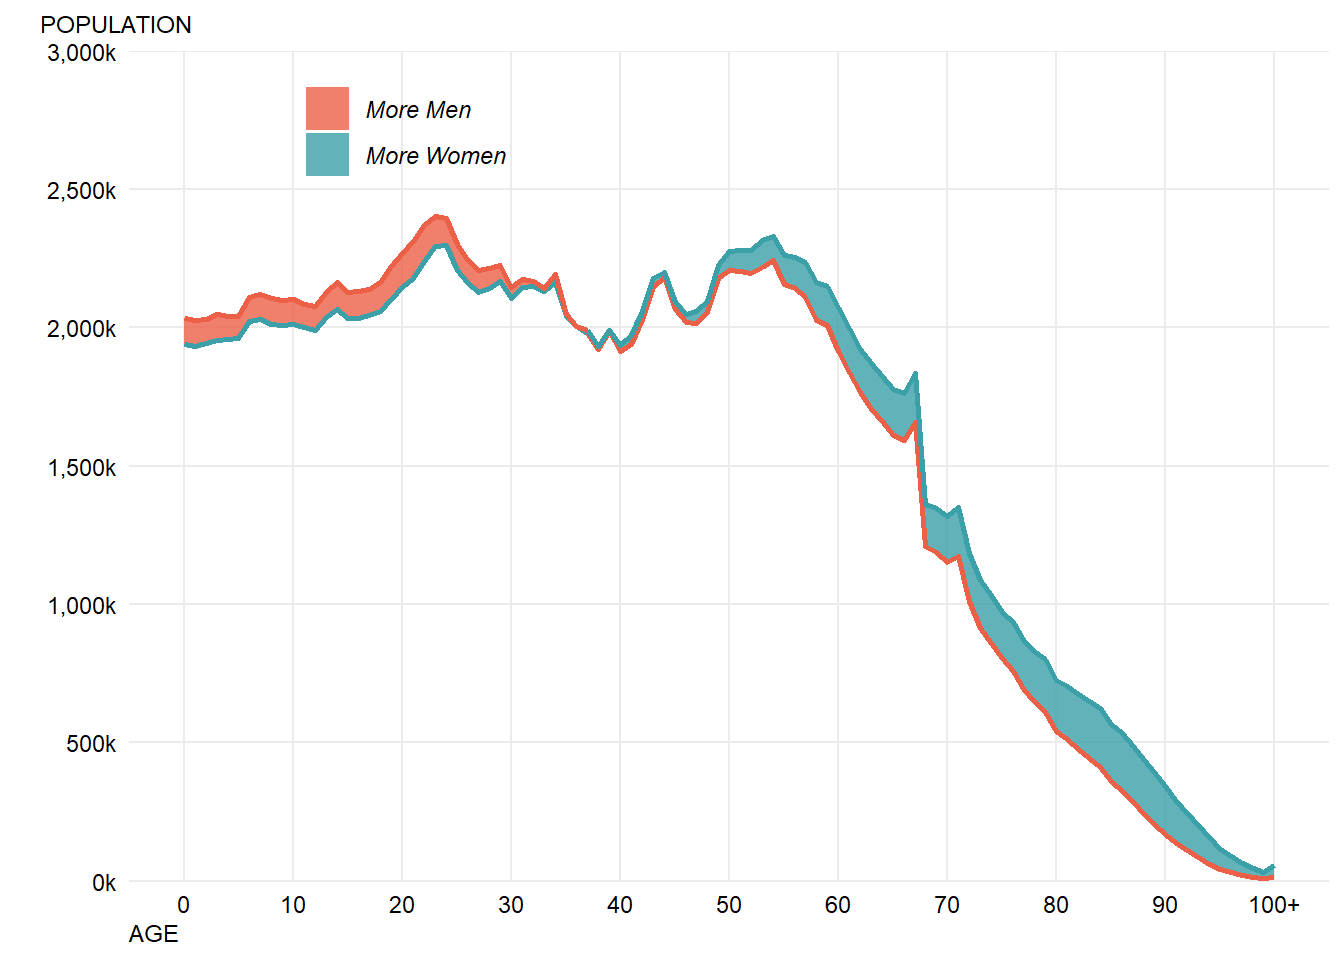
\includegraphics{2018-10-25-replicating-flowingdata-population-charts-in-r_files/figure-latex/unnamed-chunk-20-1.png}

Before getting to animation there are two more missing formatting points
- the solid x-axis line and the year value.


\end{document}
